\section{Introduction}


\begin{figure*}
  \centering
  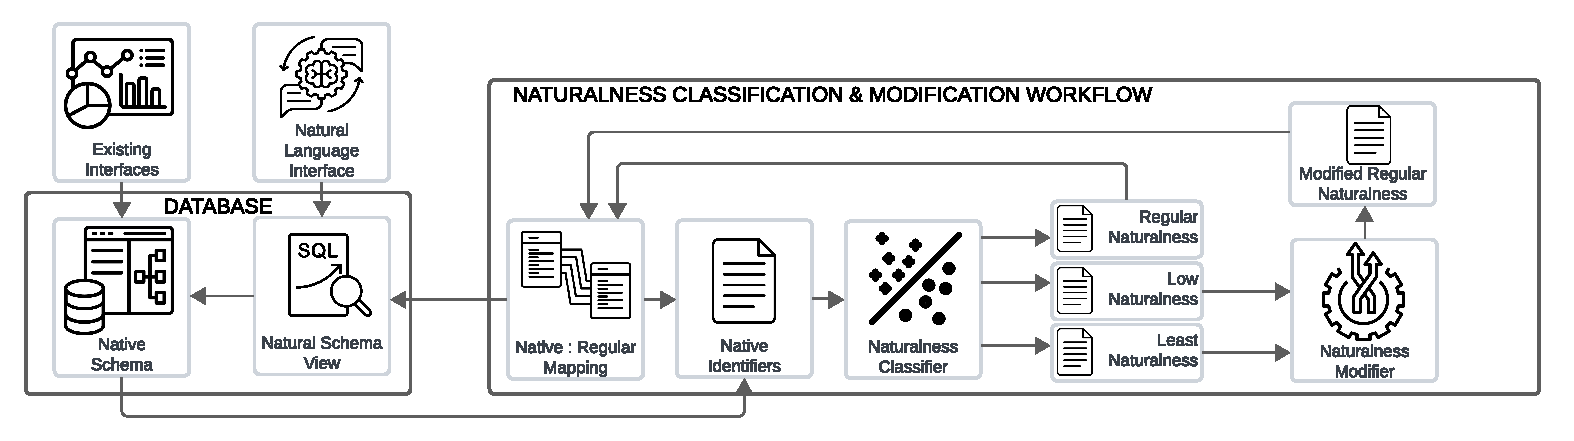
\includegraphics[width=\linewidth]{figures/Naturalness Pipeline - modification_workflow.pdf}
  \caption{Databases with poorly named, or less natural, schema identifiers perform poorly in LLM-based NL-to-SQL interfaces, and this project exposes the need for more natural schemas. We offer approaches and artifacts, including a naturalness classification and modification workflow, that can aid in the naturalness assessment and modification processes required to create a performance-enhancing natural view. In this way, the native schema remains as-is so that existing tools can continue talking to it without modification, while an LLM-based NLI can be integrated into the existing stack via a natural view.}
  \label{fig:artifact-map}
\end{figure*}

Natural language-to-SQL (NL-to-SQL) query generation capability has been revolutionized by foundational large language models (LLMs)~\cite{openai-chatgpt-blog-post, roziere2023code, anil2023palm}.
This has made the integration of LLM-based query tools into relational database workflows more viable, with both established DBMS vendors and startups beginning to offer commercial NL-to-SQL interfaces.
However, challenges in the NL-to-SQL space remain that can degrade the effectiveness of an LLM-enabled data retrieval workflow in real-world databases~\cite{floratou2024nl2sql}.
Principal among such challenges is \emph{schema linking}, which is the association of entities in NL utterances to elements in the database schema.

While much work has studied making LLMs larger or more sophisticated, a more basic issue often underlies this challenge: lexical mismatches between natural language and poorly-named tables and columns in a schema.
Intuitively, schema elements that are ``better named'' could raise the accuracy of schema linking within the NL-to-SQL setup.
In this paper, we unpack and dive deeper into this intuition to study how exactly the ``naturalness'' of schema elements matters for NL-to-SQL by instituting a new benchmark and performing extensive empirical analysis using that.
One might ask: \emph{Why bother formalizing a concept that seems obvious and intuitive?} 
We believe this is important for 2 reasons.
First, without a more formalized--or at least automated way--to define, verify, and compare ``naturalness'' researchers and practitioners alike will be forced to grapple with ad hoc and inconsistent approaches. 
In turn, this can lead to confounded conclusions by researchers on how different LLMs behave on different schemas and mislead practitioners comparing different NLIs. 
This points to the need for a new benchmark labeled dataset for this problem.

Second, practitioners need a way to efficiently and accurately operationalize any insights about the impact of naturalness on their schema elements for LLM-based NLIs.
This points to the need for a systematic evaluation of how naturalness affects different databases, queries, and LLMs used for NL-to-SQL.

\paragraph{\textbf{Our Focus}}

In this paper, we take the first steps toward deeper understanding on this seemingly obvious, but hitherto underexplored and important, relationship between schema identifier naturalness and LLM-based NL-to-SQL.
Specifically, we ask the following three interconnected questions.
(1) How do we quantify ``naturalness'' of schema identifiers? (2) Does it really impact schema linking accuracy in LLM-based NL-to-SQL and if so, by how much? (3) How does that impact vary by complexity of the database and query, as well as across different popular LLMs?

To answer the above questions, we create a novel integrated benchmark suite we call SNAILS with new collections of real-world databases and query pairs, a new labeled dataset of schema identifiers, a set of evaluation metrics, and LLM prompting and other AI artifacts.

\subsection{Preliminaries and Setup}

\paragraph{\textbf{LLM-based NL-to-SQL}}

The most obvious way to seek LLM performance improvements would be by increasing the power of the language models themselves. 
But the cost of training and deploying LLMs continues to increase in concert with their complexities. 
Additionally, many practitioners seek ``plug and play'' solutions by employing already-available LLMs. 
Model training and finetuning impose access barriers that may render such a pursuit untenable for organizations that use databases but lack the requisite talent such as data science and machine learning expertise.

The practice of prompt engineering can also help improve NL-to-SQL performance, 
though dealing with schema complexity and schema representations in LLM prompting is an ongoing challenge in enterprise-level NL-to-SQL applications~\cite{floratou2024nl2sql}.
The majority of leading submissions on the popular Spider NL-to-SQL benchmark leaderboard are LLM-based solutions~\cite{gao2023texttosql,pourreza2023dinsql,dong2023c3} that employ a variety of prompting strategies, some of which require multiple successive API requests containing schema context and instructions.
These approaches can be costly and unintuitive for NLIDB end users, and can incur excessive costs and overhead when deployed at scale. 

A complementary line of work on realistic NL-to-SQL benchmarking uses structural schema modification such as normalization, flattening, and replacement to evaluate effects on LLM performance.
Making such structural changes to target schemas challenges model robustness and increases error rates in NL-to-SQL performance~\cite{10.14778/3494124.3494139}, and this recent work indicates that schema design is a viable target for LLM-based NL-to-SQL accuracy improvements.

\paragraph{\textbf{Schema Linking}}

Schema linking remains as a persistent challenge for LLMs.
With the availability of capable LLMs that consistently generate valid SQL statements, a larger proportion of NL-to-SQL generation errors are now associated with incorrect or ambiguous database identifier selection as opposed to incorrect syntax~\cite{49288}.
Schema linking performance has been improved using lexical matching heuristics~\cite{10023434, 10096170}, joint relationally aware embeddings with attention~\cite{wang2020rat-sql, cao-etal-2021-lgesql}, the use of pre-trained language models to perform schema probing~\cite{10.1145/3534678.3539305}, and multimodel pipelines with ML models for pruning schema knowledge~\cite{li2023resdsql}.
Some NL-to-SQL methods address schema linking challenges by adding additional context such as sample values or metadata~\cite{pourreza2023dinsql} to schema knowledge representations.
These methods can improve performance in some cases~\cite{nan2023enhancingfewshottexttosqlcapabilities}, and can be useful for schemas with obscurely-named tables and columns, though they do so at the cost of much larger schema knowledge representations.


Schema linking still often fails, even with the most capable LLMs due to poorly-aligned schema identifier names with natural language question contents, that could be due to the use of synonyms or the obscurity of a database identifier.
In the latter case, it can be challenging for even a sophisticated linking solution to match natural language words to schema elements that yield minimal semantic meaning.

\paragraph{\textbf{Schema Naming Conventions}}

The majority of database schema naming best practices originate from \emph{practitioners} and are generally published as software documentation, organization policies, tutorials, etc. 
We find that there is a gap in database and data integration \emph{academic} literature evaluating schema identifier naming practices for any purpose.
While the semantics of schema identifiers may not have been considered as a necessary subject of database research in the past, the increasing integration of natural language interfaces to databases has elevated its importance.

Naming conventions for database schema identifiers vary by organization, database vendor, application, and purpose.
A web search for database table and column naming guidelines yields multiple resources ranging from blog posts~\cite{csharp-naming-convention}, 
StackOverflow responses~\cite{stackoverflow-naming-convention}, DBMS vendor documentation~\cite{oracle-schema-naming-guidelines}, and tutorials~\cite{inbo-naming-convention}.
Poor schema identifier naming practices is considered a database code smell~\cite{10.1145/3183519.3183529} where meaningless identifier names should be avoided.
Generally, the most consistent best practices include selecting descriptive and concise names that contain only commonly-understood abbreviations and acronyms, though some conventions suggest the use of abbreviated prefix and suffix modifiers that describe application associations, or entity purpose~\cite{oracle-schema-naming-guidelines-2}.

In our research, we identified several databases containing schemas with varying levels of human-readability and understandability (what we will call naturalness) which suggests that there can be a tendency for database schema designers to choose shorter and less descriptive identifier naming conventions.
As we will see, such naming shortcuts can negatively affect NL-to-SQL performance.

\subsection{Our Benchmark Artifacts and Analyses}
Given the above context of our benchmarking setup, we now explain the new artifacts in SNAILS, followed by a summary of our empirical analysis.

\paragraph{Artifact 1: Real-World Database Schemas}
The SNAILS benchmark contains several new \emph{real-world database schemas} that are not part of existing NL-to-SQL benchmarks (Artifact 1).
Our focus on schema naming motivates the creation of a new novel benchmark dataset, because existing benchmark naturalness levels are higher than those of many real-world schemas, and other real-world schema collections including SchemaPile~\cite{doehmen2024schemapile} lack the necessary database instances to enable NL-to-SQL evaluation.
In our analysis of these real-world schemas, we discover that identifier naming variances generally appear in the form of abbreviations and expansions; we refer to these variances as identifier \emph{naturalness}.

\paragraph{Artifact 2: Identifier Naturalness Classifications}
Our analysis reveals that naturalness can be formalized categorically with the help of finetuned language models and feature engineering.
We then hand-label the schema identifiers, with some ML assistance, to classify their naturalness level and produce a new golden labeled dataset.
We classify identifiers into one of 3 naturalness levels (Regular, Low, and Least) (Artifact 2).
This dataset, consisting of over 17,000 labeled identifiers, serves as the training data for the naturalness classifiers described next.

\paragraph{Artifact 3: Naturalness Classifiers}
We experiment with various classification approaches, and make available the models trained to classify the naturalness of a database schema identifier (Artifact 3).

\paragraph{Artifact 4: Naturalness-Modified Identifiers}
To better understand the effect of schema identifier naturalness, and to enable within-database experiments, we create alternate versions of each real-world schema identifier at each naturalness level (Artifact 4).
This dataset serves two purposes: 1) Training data for ML-based naturalness modifiers, and 2) Generation of schemas with varying naturalness levels to analyze the impact of naturalness on NL-to-SQL performance.
We modify the identifiers with the assistance of LLM prompting, finetuned models, and database metadata.

\paragraph{Artifact 5: Naturalness Modifier}
We offer an in-context learning-based prompting strategy for identifier naturalness reduction (or abbreviation).
We also provide an identifier naturalness increaser (or expander) that leverages retrieval augmented generation, interactive few-shot example building, and database metadata parsing methods to streamline the database naturalness improvement process.

\paragraph{Artifact 6: NL-to-SQL Question Query Pairs}

The SNAILS benchmark contains 503 NL question-SQL query pairs which we use for NL-to-SQL performance analysis of 4 LLMs.
We created this new collection as another hand-labeled golden dataset without the use of AI-based workflows (Artifact 6).

\paragraph{\textbf{Experimental Evaluation}}

Using the SNAILS benchmark artifacts, we analyze and experiment with the effects of schema identifier naturalness on LLM NL-to-SQL performance.
We select 5 publicly-available LLMs: OpenAI's GPT-3.5, GPT-4o, a finetuned variant of Meta's Code-Llama, Google's newest Gemini 1.5, and CodeS finetuned for NL-to-SQL. We evaluate them using both execution result set matching and a novel identifier set comparison approach that pinpoints schema linking performance.

In this paper we focus primarily on a simple zero-shot prompting of the LLM for our experiments.
We recognize that this may not be the best for overall execution accuracy, but it helps us isolate the impact of schema identifier naturalness in this first work on this problem.
As such, more complex workflows will create confounding effects while not necessarily providing more insights into schema linking performance.
However, for completeness sake, we also compare two illustrative complex workflows: DIN SQL for task-specific prompt chaining~\cite{pourreza2023dinsql}, and CodeS~\cite{10.1145/3654930} for NL-to-SQL finetuning.

We find that schema identifier naturalness by and large does have a meaningful effect on NL-to-SQL accuracy and schema linking performance.
Specifically, identifier naturalness is moderately and positively correlated with both schema linking and execution accuracy.
Identifiers of low naturalness yield lower performing NL-to-SQL inferences in terms of both schema linking (identifier recall) and execution accuracy.
These findings have implications for practitioners who are either designing new databases intended for LLM-based applications, or seeking to augment existing RDBMSs with an LLM-based NL-to-SQL interface.

In summary, this paper makes the following contributions:
\begin{itemize}
  \item We propose a novel measure of \emph{naturalness} of a database schema identifier and demonstrate through extensive experiments that naturalness has a significant effect on LLM schema linking performance in the context of NL-to-SQL.
  \item We provide a hybrid LLM-generated and human-curated training dataset (Artifact 2) and language model (Artifact 3) for schema naturalness classification.
  \item We offer a new multi-domain NL-to-SQL evaluation benchmark collection consisting of 9 real-world relational databases (Artifact 1) and 503 unpublished NL-to-SQL query pairs (Artifact 6) that do not exist in any LLM training corpora.
  \item We create a novel labeled dataset of alternate naturalness levels that map the identifiers from Artifact 1 to hybrid LLM-human curated identifiers of different naturalness levels (Artifact 4), and methods for expanding and abbreviating identifiers to change their naturalness (Artifact 5).
  \item We conduct an extensive empirical analysis of the performance of 5 popular foundational LLMs over our benchmark using a novel schema linking metric for NL-to-SQL.
  \item We propose a realistic workflow that enables the preservation of existing database integrations while offering LLM-based NLIs a natural view of a target schema.
\end{itemize}

% 
\section{Background}



\section{Schema Identifier Naturalness}


Intuitively, naturalness can be thought of as the degree to which a phrase, or word, resembles natural language. 
Naturalness is a concept and target of research in field of controlled natural languages~\cite{10.1162/COLI_a_00168}, where controlled language syntax is evaluated in terms of naturalness levels. 
Recent NL-to-SQL research also defines and measures naturalness~\cite{10.14778/3494124.3494139} for the purpose of evaluating the naturalness of natural language question utterances, but avoids measuring the naturalness of schema elements.

To the best of our knowledge, no prior attempts have been made to definitively measure the naturalness of a database schema's identifiers.
In order to achieve this goal, we propose a three-category naturalness classification scheme in order to measure the effects of naturalness on NL-to-SQL performance.

\subsection{Naturalness Categories}
\label{section:naturalness-categories}

\begin{figure}
  \centering
  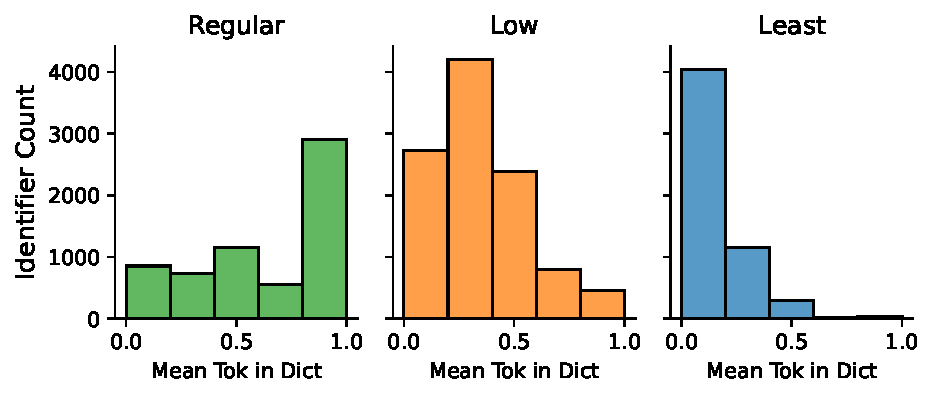
\includegraphics[width=\figwidthmod\linewidth]{figures/mean_token_in_dictionary.pdf}
  \caption{\emph{Mean Token in Dictionary}, the proportion of tokens in an identifier that match a word in an English dictionary, generally aligns with the SNAILS 3-class naturalness categorization approach.}
  \label{fig:meantokenindictionary}
\end{figure}

\begin{table}[t]
  \centering
  \begin{tabular}{|p{3.5cm}|p{2.1cm}|p{2.1cm}|}
  \hline
  \textbf{Regular} & \textbf{Low} & \textbf{Least}\\
  \hline
  airbag & AccountChk & AdCtTxIRWT \\
  AdaptiveCruiseControl & IsueFrDate & COGM\_Act \\
  ModelYear & RecvAsst & DfltSlp \\
  service\_name & UsrQuery & FNDAbs \\
  Research\_Staff & ValueOfT & CSI22 \\
  \hline
  \end{tabular}
  \caption{Example identifiers and their naturalness levels, from the SNAILS naturalness labeled dataset\\ (Artifact 2).}
  \label{table:nat-cat-examples}
\end{table}

As the first work on this topic of how schema identifier naturalness affects LLMs, we seek to define a preliminary metric--one that is consistent and descriptive enough to differentiate between naturalness levels and to measure their effects.

To gain insights into naturalness-related trends in the SNAILS datasets, we create a \emph{mean token-in-dictionary} measurement that describes the proportion of tokens in an identifier that exactly match a word in a comprehensive English word list.
Figure \ref{fig:meantokenindictionary} reveals differences between each naturalness category where Least naturalness identifiers contain fewer in-dictionary tokens, and Regular naturalness identifiers are more likely to consist of in-dictionary tokens.
This distribution suggests that because the bulk of the training corpora of LLMs is human-generated natural language text, what humans consider ``natural'' for such identifiers generally aligns with how LLMs react to them.

Examples of schema identifiers and their naturalness categories are displayed in Table \ref{table:nat-cat-examples}.
We define these categories with the underlying assumption that the identifiers are named as some semantic representation of the data, and that naming-related problems of interest are related how an identifier is codified.
That is, identifiers are assumed to not be random character sequences or random words that do not correspond to the content of the database entities they represent.
With this assumption in mind, we categorize naturalness into 3 discrete levels as follows: 
\begin{itemize}
  \item Regular: The identifier contains complete English words with no abbreviations or acronyms, or contains only acronyms in common usage (e.g., ID or GPS).
  \item Low: The identifier contains abbreviated English words and less common acronyms that are usually recognizable by non-domain experts (e.g., UTM or  CPI). The meaning of the identifier can be inferred without consulting external documentation.
  \item Least: The identifier's meaning cannot be inferred by non-experts due to indecipherable acronyms or abbreviations, and external metadata or other documentation must be consulted in order to determine its purpose.
\end{itemize}

While we recognize that naturalness can also be treated as a continuous spectrum, between the choices of continuous scoring and discrete categories, we select the latter as an initial approach to naturalness evaluation.
The primary factors underlying this choice are the level of effort required to conduct human-based scoring of a large set of database identifiers, and the difficulty of consistently scoring naturalness on a continuous range over a large set of data.
Therefore, we use an intuitive and easily-verifiable discrete 3-class taxonomy in the first work on this topic.


\subsection{Naturalness Classification}
\label{subsection:naturalness-scoring}




To consider naturalness as a factor in NL-to-SQL performance, we derive naturalness scores of the target schemas' identifiers.
We use this score to consider effects of individual identifier naturalness, schema naturalness, and query identifier naturalness.
Because manual naturalness classification can be a time consuming task for large schemas, we automate the process by training a machine learning-based classifier.
This effort is beneficial in multiple situations.
First, it can ease some manual effort of the labeling process and make the process of scaling to more databases in the future less labor intensive.
Second, it can help practitioners efficiently and consistently evaluate the naturalness of their own database schema identifiers prior to NLI integration.


To train a classifier to perform identifier naturalness scoring, we employ the 3-class set of naturalness categories described in Section \ref{section:naturalness-categories}, and a list of database identifiers drawn from the SNAILS real-world database schemas (Artifact 1).
We categorize the naturalness of each identifier to generate the SNAILS \emph{identifier naturalness classification} labeled data (Artifact 2) which we use for ML-based naturalness classifier training, evaluation and testing.

We evaluate multiple classification approaches including heuristic-based word matching, few-shot LLM prompting with GPT-3.5 and GPT-4, and LLM finetuning.
The GPT-4 few-shot approach achieves 74 percent accuracy and an f1 score of 0.77.
We experiment with multiple finetuning collections, first using a hand-labeled collection of 1,648 naturalness classifications and then leveraging the initial classifier along with weak supervision to generate a larger collection of 17,226 labeled identifiers.
Finetuning using the second collection outperforms all few-shot approaches, with the
two best-performing classifiers fine-tuned GPT 3.5 and BERT-based CANINE~\cite{Clark-2022} models performing at 89 percent accuracy, and 0.89 f1 score.

\begin{figure}
  \centering
  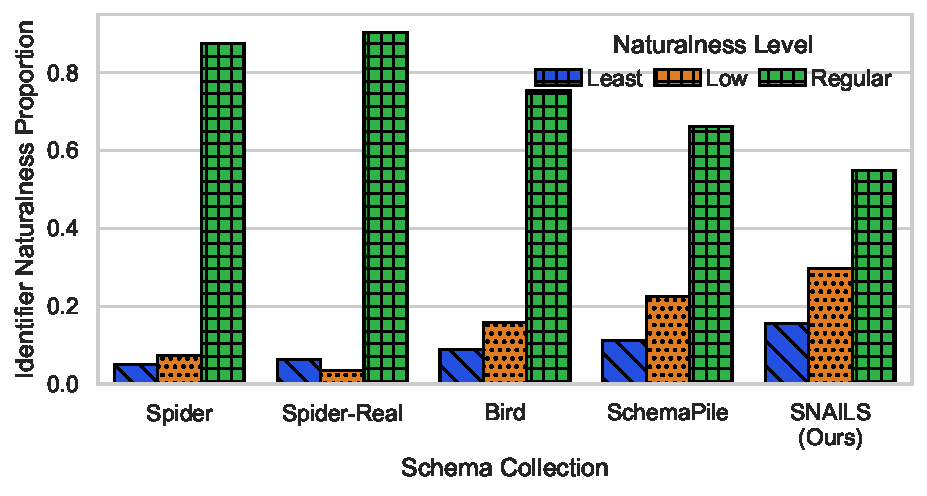
\includegraphics[width=\figwidthmod\linewidth]{figures/benchmark_naturalness_compare.pdf}
  \caption{Comparison of the SNAILS database collection (Artifact 1) described in Section \ref{subsection:benchmark-datasets} to other real-world and benchmark schema collections. SNAILS naturalness proportions are generally biased toward less natural identifiers and is more consistent with the real-world SchemaPile collection than other existing benchmarks including Spider and Spider Realistic.}
  \label{fig:naturalnesscompare}
\end{figure}

\begin{figure}
    \centering
    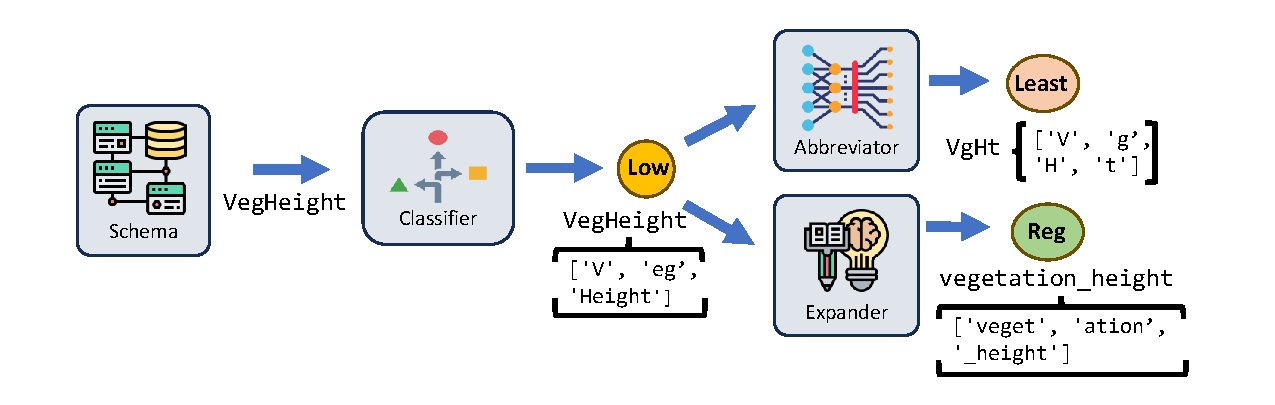
\includegraphics[width=\linewidth]{figures/classify-modify-pipeline.pdf}
    \caption{Schema identifiers are classified (Artifact 2) and modified to increase or decrease naturalness as appropriate. Modified identifiers comprise the schema crosswalks used for schema modification during NL-to-SQL experimentation (Artifact 3).}
    \label{fig:classify-modify-pipeline-main}
\end{figure}

Figure \ref{fig:naturalnesscompare} provides a visual comparison between the SNAILS schema collection and common NL-to-SQL benchmarks including Spider, Spider Realistic, and BIRD.
Additionally, we compare the SNAILS collection to the real-world SchemaPile collection and find that SNAILS collection proportions generally align to SchemaPile naturalness, more so than other existing benchmarks, which creates a more realistic and challenging benchmark in terms of schema naturalness.

To better understand the magnitude of naming practices in real-world schemas,
we use the CANINE-based classifier to classify the naturalness of the SchemaPile collection: a large volume of real-world database schemas~\cite{doehmen2024schemapile} that contains over 22,000 database schemas, 198,000 tables, and 1 million columns.
We find that in over 7,500 schemas (32 percent of the collection) Least natural identifiers make up at least 10 percent of the schema identifier names.
Additionally, over 5,000 schemas register a combined naturalness of 0.7 or below--an indicator that the schema contains a high level of Low and Least naturalness identifiers.
We examined the naturalness category distribution for these 5,000 schemas, and found that for this subset of schemas Low and Least naturalness identifiers outnumber Regular naturalness identifiers.
These findings reinforce the importance of the naturalness problem by confirming that, although a reasonable majority of schemas are already natural, there still exist many schemas with lower naturalness levels in the real-world--enough to motivate the formalization of schema naming quality measures.


\subsection{Identifier Schema Naturalness Mapping}
\label{subsection:naturalnessmapping}

In addition to measuring the effects of identifier naturalness in existing schemas, we also seek to evaluate the effects of modifying schema naturalness.
For this purpose, we create Artifact 4, naturalness-modified identifiers.
This artifact enables schema modification during prompt generation and query inference, which provides a within-schema assessment of naturalness level effects on NL-to-SQL accuracy.

\paragraph{\textbf{Identifier Mapping}}
In addition to the ground truth, or Native, naturalness of the 9 schemas in the SNAILS real-world database collection, the naturalness-modified identifier collection contains 3 additional sets of identifiers: Regular, Low, and Least.
That is, each native identifier is mapped to 2 additional, semantically equivalent, identifiers of higher or lower naturalness, and mapped to itself for its own naturalness level (i.e., we do not generate new identifiers of the same naturalness as its native form).



Figure \ref{fig:classify-modify-pipeline-main} provides a visual example of the Native identifier \emph{VegHeight} which is classified as Low naturalness.
With this naturalness classification as a starting point, we abbreviate it further to generate a corresponding Least naturalness identifier \emph{VgHt}.
We also expand it to generate the corresponding Regular naturalness version \emph{vegetation\_height}.
We map the Native \emph{VegHeight} identifier to itself in the Low naturalness category.

\paragraph{\textbf{Naturalness Modification}}
For \emph{more natural to less natural} modifications (the abbreviator in Figure \ref{fig:classify-modify-pipeline-main}), we employ in-context learning (few-shot) prompt strategies with GPT-3.5 turbo to generate naturalness-modified identifiers (e.g., Regular to Low, Low to Least, and Regular to Least).
We favor this approach over model finetuning, as simple instructions to abbreviate the identifier coupled with several examples prove more effective and less prone to poor results (e.g., presence of unwanted characters in the modified identifier).

Automating the reverse \emph{less natural to more natural} naturalness modification (the expander in Figure \ref{fig:classify-modify-pipeline-main}) requires additional context and external knowledge from data description sources.
Though a recent project describes a promising identifier expansion strategy~\cite{nameguess} without external knowledge, it requires finetuning over a large dataset, and is likely susceptible to overfitting; therefore we opt for our own approach that incorporates the use of an LLM augmented with schema metadata lookup capability.
To accomplish this, we create a Python program with GPT interaction that takes as input metadata describing a schema's native identifiers, and outputs an identifier with regular naturalness.
More details of this process are available in the \iftechreport{appendix}\else{technical report~\cite{techreport}}\fi.


\section{Base Collections}


Given the recency of the LLMs selected for evaluation in this project, and the relative maturity of existing NL-to-SQL benchmarks, we believe that foundational LLMs have been exposed to existing benchmark training and development NL questions and queries in their training corpora.
NL-to-SQL performance differences between queries over seen vs. unseen schema are significant~\cite{49288}, and we seek to avoid as much bias as possible due to intentional or unintentional pre-training on existing benchmark datasets.

We also find that existing benchmarks including Spider~\cite{Yu&al.18c}, and BIRD~\cite{li2023llm}, do not match the identifier naturalness distribution of real-world schema collections such as SchemaPile~\cite{doehmen2024schemapile}.
Although SchemaPile is a very large representation of real-world schemas, it does not contain database instances necessary for benchmark performance evaluations; so, we are not able to leverage its dataset in the creation of a new benchmark.
To reduce bias due to benchmark data exposure, and to create a benchmark more representative of real-world schema naming, SNAILS contains two artifacts for NL-to-SQL benchmarking: Artifact 1, which is a collection of 9 publicly-available database schemas and data; and Artifact 6, a human-generated set of 503 NL question - gold query pairs.

\subsection{Datasets}
\label{subsection:benchmark-datasets}

\begin{table}[t]
  \centering
  \begin{tabular}{|p{2cm}|c|c|c|c|}
  \hline
  \textbf{Database} & \textbf{Tables} & \textbf{Columns} & \textbf{Questions} & \textbf{Org} \\
  \hline
  ASIS & 36 & 245 & 40 & NPS \\
  ATBI & 28 & 192 & 40 & NPS \\
  CWO & 13 & 71 & 40 & NPS \\
  KIS & 18 & 157 & 40 & NPS \\
  NPFM & 27 & 190 & 40 & NPS \\
  NTSB & 40 & 1611 & 100 & NHTSA \\
  NYSED & 27 & 423 & 63 & NYSED \\
  PILB & 21 & 196 & 40 & NPS \\
  SBOD & 2588 & 90,477 & 100 & SAP \\
  \hline
  \end{tabular}
  \caption{SNAILS Real-World Database Schemas}
  \label{table:benchmarkschemas}
\end{table}

\paragraph{\textbf{Native Schemas}}
The SNAILS real-world database schema collection (Artifact 1) consists of 9 databases sourced from multiple locations.
We refer to the schema identifier names as they exist in the source databases as \emph{Native}, and we classify each schemas' Native naturalness level (see Figure \ref{fig:databasenaturalness}).
Domain diversity facilitates a more thorough evaluation~\cite{finegan-dollak-etal-2018-improving}; so, SNAILS database collections span multiple domains.
Domain coverage includes scientific nature observation records, vehicle safety statistics, primary school performance data, and business resource planning.

The U.S. National Parks Service's IRMA Portal~\cite{nps-irma-portal} is the source of the scientific observation databases which include the 
Field Data for the Inventory of Amphibians and Reptiles of Assateague Island National Seashore (\textbf{ASIS})~\cite{assateague-herp}, 
Great Smoky Mountains All Taxa Biodiversity Inventory (\textbf{ATBI}) Plot Vegetation Monitoring Database~\cite{gsmnp-atbi}, 
Wildlife Observations Database: Craters of the Moon National Monument and Preserve 1921-2021 (\textbf{CWO})~\cite{craters-of-the-moon-wildlife}, 
Exotic and Invasive Plants Monitoring Database (\textbf{KIS})~\cite{klamath-inventory}, 
Northern Plains Fire Management (\textbf{NPFM})~\cite{ngp-fire}
and Pacific Island Network Landbird Monitoring Dataset (\textbf{PILB})~\cite{pilb-dataset}. 

The National Transportation Safety Bureaus 2021 safety sampling dataset~\cite{ncsa2022overview, crash-investigation-sampling-system} is the source of SNAILS \textbf{NTSB} safety statistics database. 
We source school performance data (\textbf{NYSED}) from the New York State Education Department~\cite{nysed-report-card}. 

The business resource planning database \textbf{SBOD} is a training example of the popular SAP Business One system, and is publicly available in MS SQL server backup format~\cite{sap-demo}.
The SBOD schema consists of an extremely large number of tables and columns; so pruning is required to fit the schema within the context window of the LLMs we compared.
We reduce the schema knowledge token requirements by segmenting the SBOD schema into submodules and further reducing tables through data profiling.
Additional information on the SBOD schema knowledge management is available in the \iftechreport{appendix}\else{technical report \cite{techreport}}\fi.

Each database was migrated from its source format into an MS SQL Server database.
Several databases contained identifiers with whitespace characters, which is uncommon in most schemas.
To mitigate whitespace-related inference failures as a confounder, we modify the native identifiers by replacing whitespace characters with underscore characters.
In total, 148 out of over 19,000 total identifiers (less than .01 percent) contained at least 1 whitespace character.

\paragraph{\textbf{Native Schema Naturalness Levels}}

Since the intent of this project is to measure the effect of schema naturalness, we first check if there is sufficient distribution of naturalness levels across the collection. 
We employ the GPT-3.5-based classifier described in Section \ref{subsection:naturalness-scoring} to evaluate the naturalness of the native schema identifiers.

In addition to measuring the proportion of identifiers in each naturalness category, we also derive a combined naturalness score.
Combined naturalness is the weighted average of category proportion values, where scores range from 0.0 to 1.0 with 1.0 representing a schema containing only Regular naturalness identifiers.
A more detailed description of its calculation is available in the \iftechreport{appendix}\else{technical report~\cite{techreport}}\fi.

Figure \ref{fig:databasenaturalness} displays the proportions of identifiers in each naturalness category, as well as the combined naturalness, in each native schema.
From the chart, we can see that the schemas in the SNAILS collection described in Section \ref{subsection:benchmark-datasets} represent a heterogeneous selection of naturalness combinations.

\begin{figure}
  \centering
  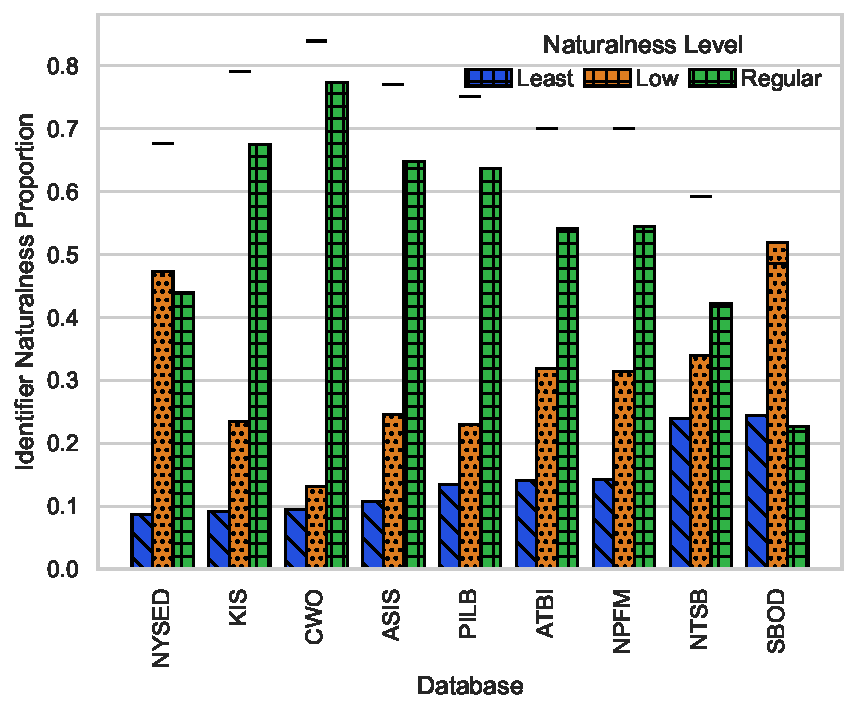
\includegraphics[width=\figwidthmod\linewidth]{figures/naturalness_by_db.pdf}
  \caption{Proportion of identifiers in each naturalness category within the SNAILS real-world database collection (Artifact 1). Horizontal line markers indicate calculated combined naturalness as described in the \iftechreport{appendix}\else{technical report~\cite{techreport}}\fi}
  \label{fig:databasenaturalness}
\end{figure}

\begin{table*}[!h]
  \centering
  \begin{tabular}{lrrrrrrrrrrrr}
\toprule
Database & Qs & Top & Funct. & Join & C-Join & Ex & SQ & Where & Neg & Grp & Ord & Hvg \\
\midrule
ASIS & 40 & 1 & 24 & 13 & 1 & 0 & 2 & 18 & 0 & 17 & 1 & 0 \\
ATBI & 40 & 5 & 20 & 18 & 0 & 1 & 7 & 21 & 2 & 16 & 7 & 1 \\
CWO & 40 & 2 & 18 & 5 & 1 & 5 & 10 & 34 & 7 & 12 & 2 & 1 \\
KIS & 40 & 8 & 26 & 15 & 0 & 0 & 2 & 25 & 1 & 11 & 8 & 0 \\
NPFM & 40 & 5 & 27 & 21 & 0 & 0 & 1 & 29 & 0 & 16 & 5 & 0 \\
NTSB & 100 & 8 & 82 & 23 & 21 & 0 & 6 & 62 & 4 & 42 & 23 & 4 \\
NYSED & 63 & 10 & 36 & 10 & 4 & 1 & 21 & 55 & 1 & 16 & 10 & 1 \\
PILB & 40 & 6 & 25 & 23 & 0 & 0 & 3 & 20 & 0 & 16 & 11 & 2 \\
SBOD & 100 & 2 & 33 & 44 & 0 & 0 & 0 & 82 & 0 & 17 & 2 & 1 \\
\bottomrule
\end{tabular}

  \caption{Gold query clause counts for each SNAILS database. Columns represent a count of gold queries that contain the listed clause types. Qs is the count of question-query pairs for each database. C-Join is the subset of joins that require a composite key. Ex indicates the use of an exists clause. SQ indicates a subquery. Neg, Grp, Ord, and Hvg represent negation, group by, order by, and having. Note: MS SQL Server dialect replaces the common LIMIT clause with an equivalent TOP clause that precedes select items in the SELECT clause.}
  \label{table:query-stats}
\end{table*}

\paragraph{\textbf{Modified (Virtual) Schemas}}
To control for confounding factors such as schema structure, normalization levels, and constraint variances between native schemas, we perform within-database evaluations of naturalness.
To accomplish this, we generate 3 additional \emph{virtual} schemas using the naturalness-modified identifiers (Artifact 4) described in Section \ref{subsection:naturalnessmapping}.
Each virtual schema is representative of a naturalness category, where schema identifiers are replaced with a semantically equivalent identifier of a different naturalness level.
This results in 4 schema versions per database in the base collection: Native, Regular, Low, and Least.

The modified schemas are virtual because we do not create database instances that can be queried directly.
Rather, we query virtual schemas via identifier replacement in prompts and generated queries using processes described in Section \ref{section:nl-to-sql-benchmarking-setup}.
This approach reduces storage overhead.
It also enables possible future schema variations of different naturalness proportions without the need to instantiate additional database instances.

\paragraph{\textbf{SNAILS Database Selection and Extension Processes}}
The initial 9 datasets and schemas are included because they were (1) publicly available, (2) not included in any prior NL-to-SQL benchmarks, (3) contained relational tables with dependencies and database instances with values, (4) had available table and column metadata, (5) represented a diversity of application domains, and (6) contain data potentially useful for real-world data analysis or data science applications.
Databases are not selected or pre-screened using perceived naturalness as criteria.

We view the initial 9 schemas as a starting point from which the SNAILS dataset can grow.
Researchers who wish to extend the SNAILS collection should use the same selection criteria.
In addition, the extension process must ensure that new databases:  (1) can be represented as MS SQL Server instances, (2) each native identifier's naturalness is classified according to defined criteria using the SNAILS naturalness classifier, and (3) that native identifiers are modified using the SNAILS modification artifacts to create alternate naturalness levels. 

\subsection{NL Question - SQL Query Pairs}

To evaluate SQL inference performance over the Native and modified schemas in the SNAILS real-world database collection, we create a new set of 503 NL-question and SQL gold query pairs (Artifact 6).
Schema identifier naturalness are the primary considerations for NL question and gold query composition.
During question and query formulation we track schema coverage to ensure that the distribution of identifier naturalness within a set of gold queries generally matches the naturalness distribution of target schemas.

To enable accuracy measurements at the identifier level, gold queries contain the minimum identifiers (tables and columns) required to answer its corresponding question.
For this reason, for questions that require the count aggregation function, where appropriate, we use the COUNT(*) clause (as opposed to selecting an arbitrary column).
This approach eliminates incorrect penalties to recall if a generated query fails to project an arbitrary column as a function argument.

Gold queries contain only native identifiers, such that all gold queries return valid non-null results from target databases in the real-world database collection (Artifact 1).
We measure query complexity as a count of its clauses and identifiers.
Gold queries span a range of complexities, from very simple single table projections, to multi-table joins and nested subqueries (see Table \ref{table:query-stats}).

\paragraph{\textbf{Adding New NL-SQL Pairs to the SNAILS Collection}}
For researchers interested in extending the SNAILS collection, it is necessary to create new ground truth NL-SQL pairs for evaluation. 
While we employed a fully manual approach for question writing, and this approach may be used for future additions, they may also consider the use of new approaches such as using a template-based approach for generating question-query pairs with relational data as input~\cite{10.5555/3666122.3667470}.
Regardless of NL-SQL pair creation method, researchers should ensure adequate schema coverage and minimum essential identifier selection as described in the preceding section.


\section{NL-to-SQL Benchmarking Setup}

\label{section:nl-to-sql-benchmarking-setup}

\begin{figure}[!h]
  \centering
  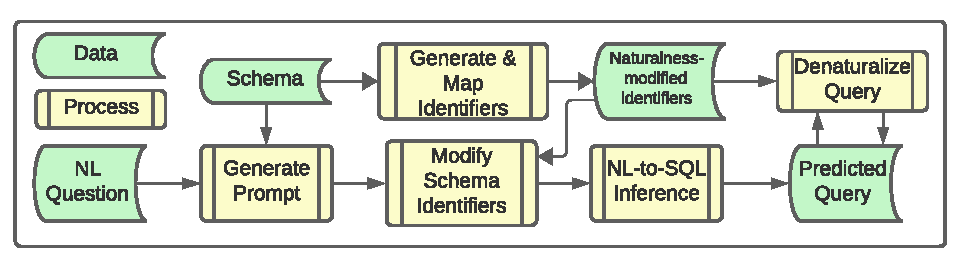
\includegraphics[width=\figwidthmod\linewidth]{figures/section-5-process-header.pdf}
  \caption{Experiment setup workflow from NL question and schema as input to predicted query as output.}
  \label{fig:section-5-process-header}
\end{figure}

To evaluate the impact of naturalness on NL-to-SQL accuracy, we build a benchmarking setup pipeline as shown in Figure \ref{fig:section-5-process-header}. 
NL question and gold query pairs, database schemas, and naturalness crosswalk mappings are inputs into subprocesses.
The subprocesses include prompt generation, schema identifier naturalness modification, identifier naturalness classification, LLM-based NL-to-SQL inference, and predicted query ``denaturalization'' (i.e., converting table and column identifiers to native schema identifiers prior to query execution).
The output of the experiment setup is a predicted query, which along with its gold query counterpart, is executed against a target database. 
This predicted query is passed into a parser analysis tool as initial steps of the \emph{Performance Evaluation and Results Classification} phase of the experiment described in Section \ref{section:nl-to-sql-benchmarking-results}.

\subsection{Prompt Generation}
The design space for LLM-based NL-to-SQL prompting is quite large, with options ranging from zero-shot instructions to sequential prompting broken into discrete tasks such as schema subsetting and error handling.
Although we evaluate 2 complex NL-to-SQL workflows, to maintain consistency across the LLMs compared in this study, our performance comparisons focus on a single prompting strategy: zero-shot prompting with schema knowledge.

\paragraph{\textbf{Prompting Strategy}}

SNAILS prompts consist of zero-shot  instructions with schema knowledge (denoted as ZS in results figures) in a format similar to OpenAI's Text-to-SQL demonstration prompt~\cite{gao2023texttosql} for completions. 
The prompt begins with task instructions and database information:

\begin{verbatim}
  For the database described next, provide only a sql query. 
  do not include any text that is not valid SQL.
  #Database: NTSB
  #MS SQL Server tables, with their properties:
\end{verbatim}

Target database system tables provide schema knowledge, which is represented as a list of tables and their column names with data types in the format:

\begin{verbatim}
  #TableName (Col1Name Type, Col2Name Type, ...)
\end{verbatim}

The prompt ends with the instruction:

\begin{verbatim}
  ### a sql query, written in the MS SQL Server dialect, 
      to answer the question: <Question>
\end{verbatim}

Where <Question> is replaced with an NL question directed at the given schema.

To evaluate naturalness effects on more complex NL-to-SQL prompting workflows, we also implement DIN SQL~\cite{pourreza2023dinsql} which uses prompt chaining with GPT-4, and CodeS~\cite{10.1145/3654930}--a multi-step NL-to-SQL system (schema filtering and SQL inference) based on StarCoder~\cite{li2023starcoder} and finetuned for the NL-to-SQL translation task.

\paragraph{\textbf{Prompt Schema Identifier Modification}}
For inference on virtual schemas with modified naturalness levels, we replace Native identifiers with corresponding identifiers of the target virtual schema's naturalness level.
We accomplish this step using the naturalness-modified identifier collection (Artifact 4) described in Section \ref{subsection:naturalnessmapping}.
We use a SQL parser to encase identifiers within tags to improve identifier replacement accuracy and eliminate errors due to substring matching between identifiers.

\subsection{NL-to-SQL Inference}

\paragraph{\textbf{Language Models}}
Foundational LLMs continue to grow in capability at a rapid pace.
Despite this growth, not all NLI implementations can avail of the most-capable LLMs, often due to organizational policy constraints (e.g., organizational security concerns~\cite{gsa-llm-directive}).
Additionally, we seek to understand if schema naming effects generalize across model architectures and sizes.
Thus, we consider several LLMs, both open and closed source, to capture as many use profiles as possible including OpenAI's GPT-3.5 Turbo and GPT-4o~\cite{openai-chatgpt-blog-post, openai-api-documentation}; Google's Gemini 1.5 Ultra~\cite{geminiteam2024gemini, geminiteam2024gemini15}; and Phind-CodeLlama-34B-v2~\cite{phind2022phindcodellama} which is a finetuned variant of Meta's CodeLlama 2~\cite{roziere2023code}.

\paragraph{\textbf{CodeS and DIN SQL Implementation}}
For the more complex DIN SQL and CodeS NL-to-SQL workflows, we provide additional versions of the SNAILS schema artifacts to conform to the input requirements of the target systems.
Additionally, we add data logging between agents to document the schema filtering step for additional analysis.
For consistency between approaches, we use GPT-4o for all steps in the prompting chain.
For CodeS inference, we execute the schema filtering and NL-to-SQL inference using the CodeS codebase and finetuned models.

\paragraph{\textbf{Generated Query Denaturalization}}
For queries targeted at virtual schemas and generated using modified schema identifiers, we perform reverse modifications prior to query execution on the native database schema.
Using a purpose-built Antlr~\cite{Parr2014}-based parser, we extract table and column identifiers, and generate a tagged query with identifier tags encasing table and column names.
The tags guide the replacement algorithm, ensuring accurate replacement of naturalness-modified identifiers with their Native naturalness counterparts.


\section{NL-to-SQL Benchmarking Results}

\label{section:nl-to-sql-benchmarking-results}

This section describes the process of evaluating the generated SQL query output from the prior section.
We evaluate performance in terms of execution accuracy (result set comparison and manual evaluation) and schema linking (recall, precision, and F1).

\begin{figure}[!h]
  \centering
  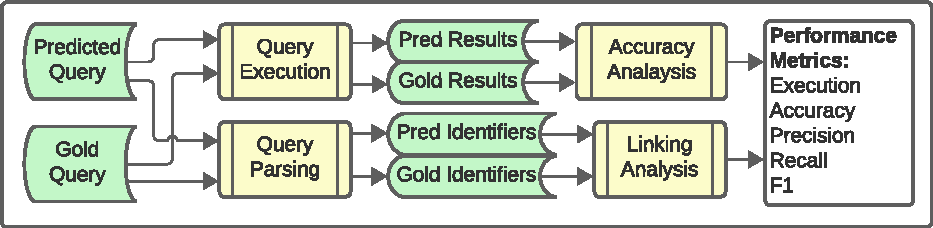
\includegraphics[width=\figwidthmod\linewidth]{figures/section-6-process-header.pdf}
  \caption{Benchmark results evaluation includes generated and gold query execution on target schemas, parser-based analysis, and identifier set comparisons. We evaluate performance in terms of execution accuracy and schema linking (precision, recall, and F1).}
\end{figure}

\paragraph{\textbf{Key Takeaways}}
Overall, there is a model-dependent statistically significant correlation between identifier naturalness and execution accuracy, with smaller models exhibiting higher correlations between naturalness and performance.
The presence of Least naturalness identifiers has the largest negative effect on schema linking.
Additionally, while the performance difference between Regular and Low is visible, it is less impactful. 
So, modifying Least naturalness identifiers should be a  higher priority than modifying Low naturalness identifiers.

\subsection{Execution Accuracy}

\begin{figure}
  \centering
  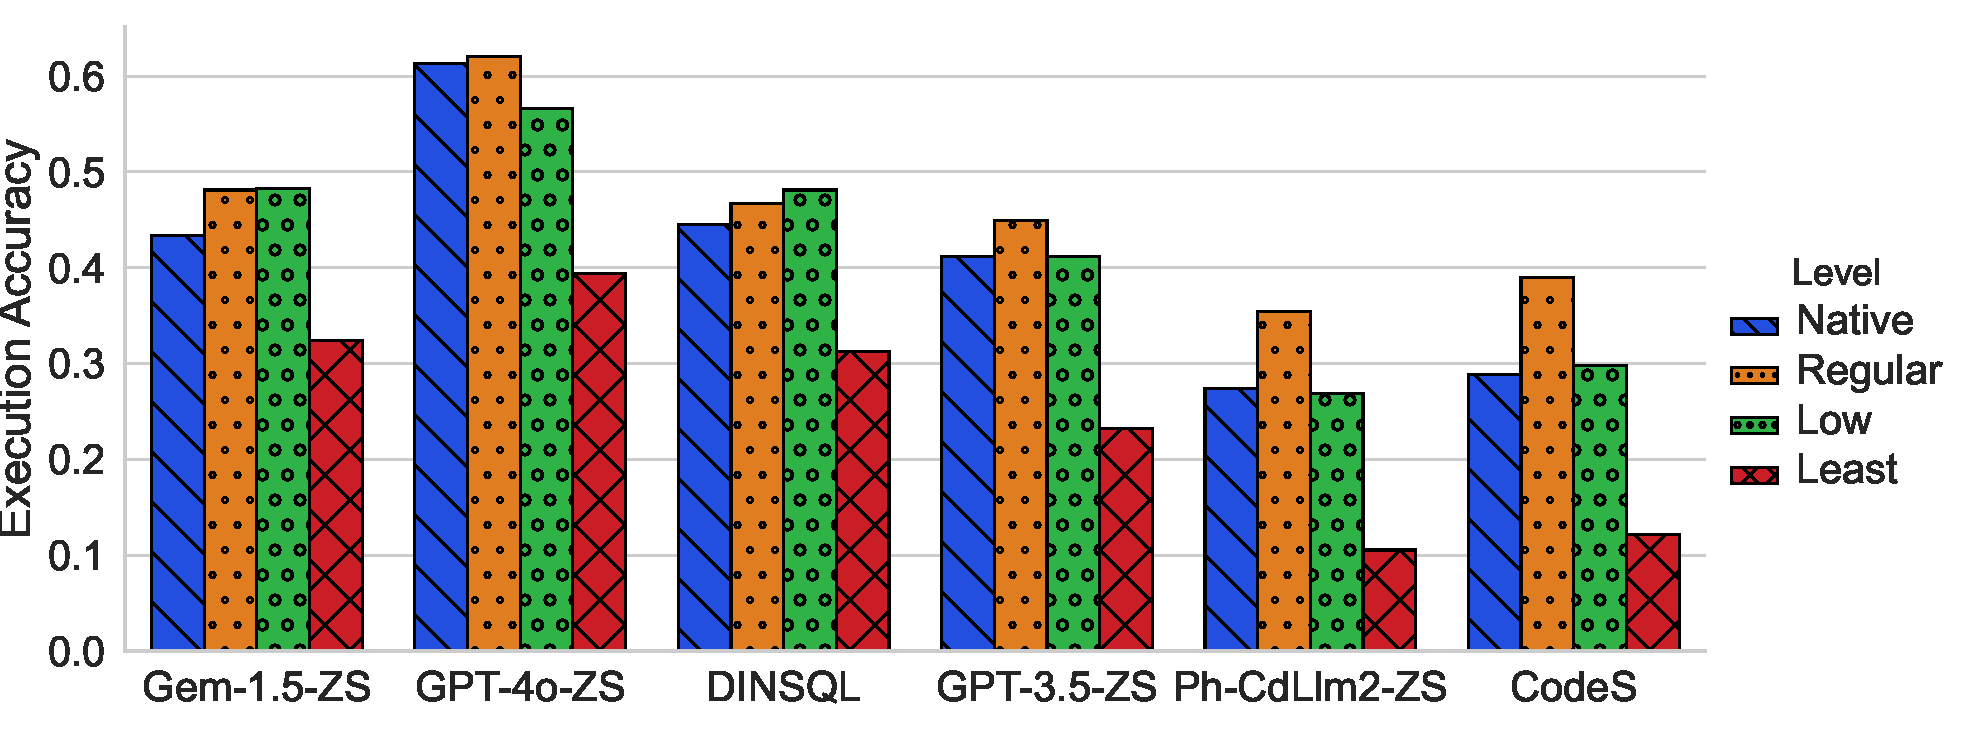
\includegraphics[width=\figwidthmod\linewidth]{figures/execution-accuracy-barplot.pdf}
  \caption{Execution accuracy (proportion of correct queries) by model. There is slight accuracy improvement from native schemas to schemas modified to regular naturalness. Accuracy drops significantly for schemas modified to low naturalness.}
  \label{fig:execution-accuracy-barplot}
\end{figure}

\paragraph{\textbf{Execution Result Set Comparison}}
Execution accuracy is the standard measure of performance in most NL-to-SQL benchmarks~\cite{li2023llm, Yu&al.18c} where accuracy is determined using result set comparisons between gold and generated queries executed over one or more database instances.
A drawback of existing methods is that strict set or bag comparisons risk increased false-negatives when a generated query includes additional fields that are not required, but do not render the result incorrect in terms of the natural language question~\cite{10023434, floratou2024nl2sql}.

To reduce false negatives, the SNAILS approach to execution accuracy evaluation adopts 2 aspects of relaxed execution matching as described in~\cite{floratou2024nl2sql}; it accounts for: (1) The possibility that a predicted query may contain additional columns beyond those retrieved by a gold query; and (2) That unless specified in the NL question, tuples may appear in any order.
To achieve this, we perform result set-superset comparisons to ensure that the predicted result set column set is a superset of the gold result set column set.
That is, a generated query is considered incorrect if it does not contain \emph{all} gold query columns; but it is not considered incorrect (at this stage) if it includes columns not present in the gold query result. 
A more detailed description of this approach is available in the \iftechreport{appendix}\else{technical report~\cite{techreport}}\fi.

\paragraph{\textbf{Manual Evaluation}}
Execution result set comparison cannot prove query correctness; so we rely on it only to rule out true negatives from further consideration.
To validate correctness, the authors manually review generated queries that pass execution result set-superset comparison checks.
We streamline this process by creating a Python-based manual validation user interface that makes the process of comparing gold and generated queries more user-friendly.
Manual validation steps include ensuring the generated query answers the NL question, matches the gold query in terms of semantic structure, and does not contain semantically incorrect predicates, projections, or clauses.

\paragraph{\textbf{Naturalness Effect on Execution Accuracy}}

Figure \ref{fig:execution-accuracy-barplot} shows execution accuracy for each LLM and naturalness level.
There is a clear difference in overall performance between LLMs, most likely due to model size.
We find that generally more natural database schemas yield more correct queries.
Databases with more natural native schemas did not benefit from identifier renaming, though we observe that altering a schema to become less natural degrades accuracy in most cases. We find that for databases with Native schema combined naturalness scores less than 0.69, modifying the schema identifiers to increase naturalness improves execution accuracy.

\paragraph{\textbf{Statistical Significance}}
The Kendall-Tau correlation between the naturalness of identifiers in a query and execution accuracy ranges from low ($\tau = 0.09, p < 0.0001$) for Gemini 1.5, to moderate ($\tau = 0.19, p < 0.0001$) for Phind-CodeLlama2 and CodeS.
The most impactful relationship is between the presence of Least naturalness identifiers and performance, with Kendall-Tau correlations between the proportion of Least  identifiers in a query and execution accuracy between $\tau=-.15$ and $\tau=-.22$ with $p < 0.0001$ for all models.

\subsection{Schema Linking Evaluation}
\label{section:linking-evaluation}

We make schema linking a ``first class citizen'' of our analysis, and study schema linking performance in queries irrespective of other aspects of correctness. 
Thus, we propose query-level and identifier-level schema linking measurements.
We propose an approach similar to the Spider benchmark exact set matching system~\cite{Yu&al.18c} in which we employ a schema linking-specific evaluation method using \emph{recall} scoring of gold and generated query pairs.
Other schema linking-focused research measure effects of schema linking improvements using ablation~\cite{wang2020rat-sql, cao-etal-2021-lgesql, 10.1145/3534678.3539305, 49288}. 
In other cases, schema linking is described in post-hoc analysis of NL-to-SQL model performance, with schema linking accounting for roughly 30\% of failures~\cite{dong2023c3, pourreza2023dinsql}.

\paragraph{\textbf{Query-Level Linking Analysis}}
The set of all schema identifiers (table and column names) present in gold queries represents the minimum identifiers required to correctly answer an NL question.
Our purpose-built ANTLR4-based~\cite{Parr2014} query parser extracts identifiers from gold and generated queries.
With a set $QI_g$ of identifiers present in the gold query and a set of identifiers $QI_p$ present in the generated (or predicted) query, we calculate recall, as well as F1 and precision.

\begin{equation}
  \label{eq:recall}
  % Recall = \frac{|I_g \cap I_p|}{|I_g \cap I_p| + |I_g - I_p|}
  QueryRecall = \frac{|QI_g \cap QI_p|}{|QI_g|}
\end{equation}

\begin{equation}
  \label{eq:precision}
  % Precision = \frac{|I_g \cap I_p|}{|I_g \cap I_p| + |I_p - I_g|}
  QueryPrecision = \frac{|QI_g \cap QI_p|}{|QI_p|}
\end{equation}

\begin{equation}
  \label{eq:f1}
  QueryF1 = \frac{2(QueryRecall*QueryPrecision)}{QueryRecall+QueryPrecision}
\end{equation}
\\
We exclude 137 linking score calculations from analysis in situations where the predicted query contains invalid SQL that prevents query parsing and identifier extraction.
We use recall as the primary measure for schema linking, as it does not penalize generated queries that contain extra identifiers that do not render an answer incorrect in our setting, such as cases when an arbitrary column is referenced in a count function.
Charts and tables depicting F1 and precision scores are available in the \iftechreport{appendix}\else{technical report~\cite{techreport}}\fi.

\paragraph{\textbf{Identifier-Level Linking Analysis}}

For an identifier-focused (rather than query-focused) metric, we perform identifier-level linking analysis.
We derive recall linking scores for each Native schema identifier $I$ as follows. 
$I_{match}$ is the count of instances when $I$ is correctly present in a predicted query. 
$I_{gold}$ is the count of gold queries that contain $I$.

\begin{equation}
  \label{eq:identifier-recall}
  IdentifierRecall = \frac{I_{match}}{I_{gold}}
\end{equation}

Figure \ref{fig:identifier-recall} visualizes \emph{IdentifierRecall} of Native identifiers in each naturalness level, and for each LLM.
The chart indicates an observable difference in \emph{IdentifierRecall} scores for each naturalness level, with \emph{IdentifierRecall} increasing for higher naturalness levels.
These results remain consistent relative to overall model performance across all 5 LLMs and various workflows.

\paragraph{\textbf{Naturalness Effect on Schema Linking}}

\begin{figure}
  \centering
  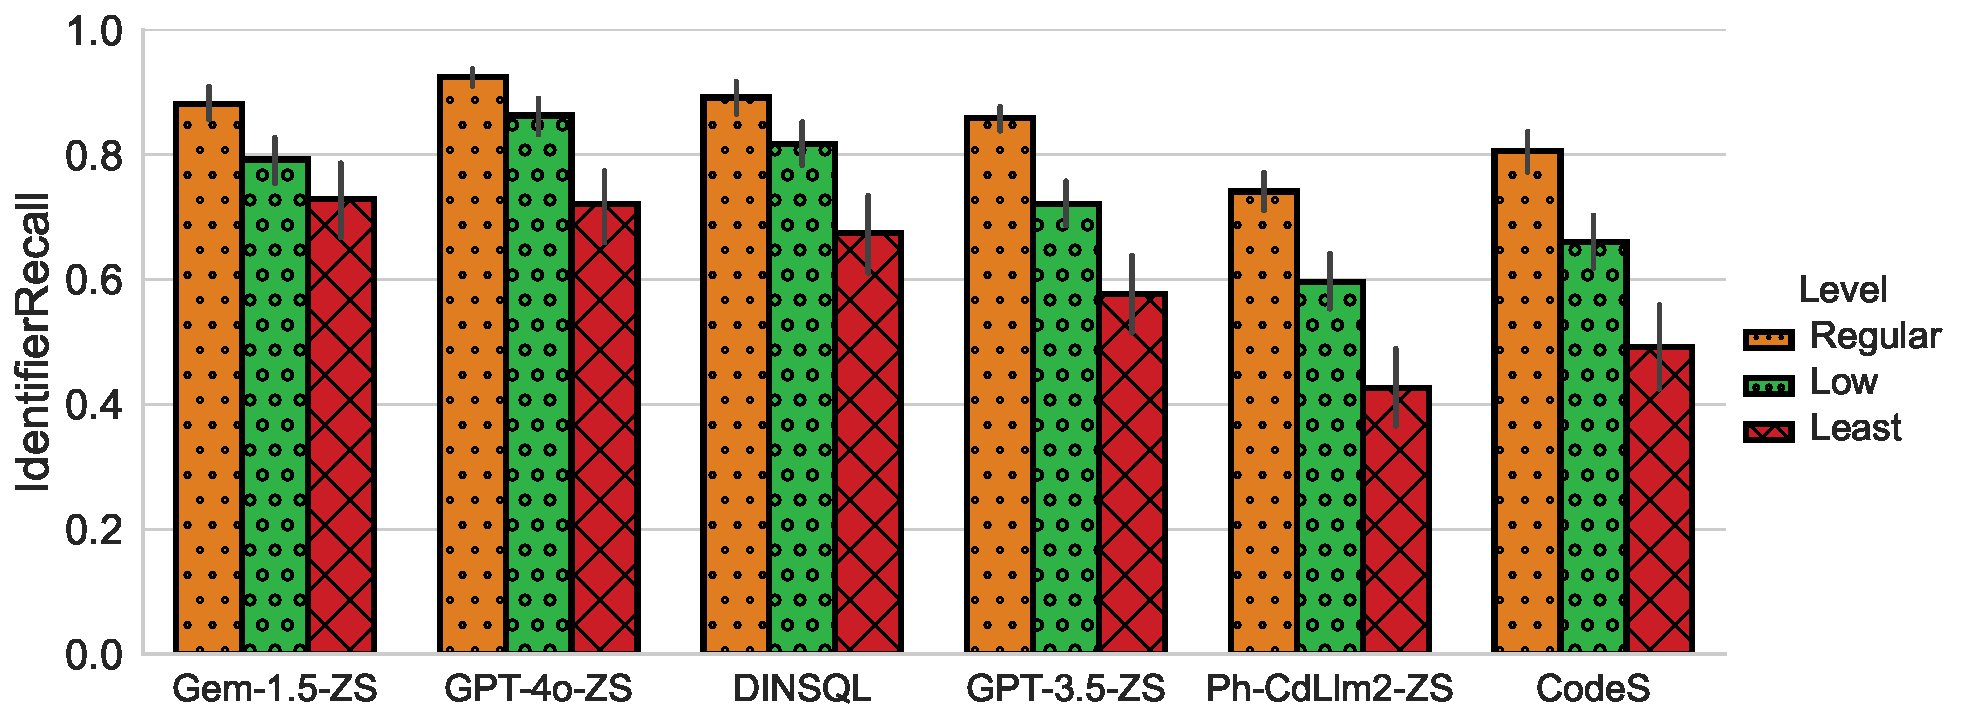
\includegraphics[width=\figwidthmod\linewidth]{figures/identifier-recall.pdf}
  \caption{Native identifier recall scores by model and naturalness level. Error bars set with confidence interval of 0.95. For all models, identifiers in lower naturalness categories yield lower recall scores.}
  \label{fig:identifier-recall}
\end{figure}

\begin{figure}
  \centering
  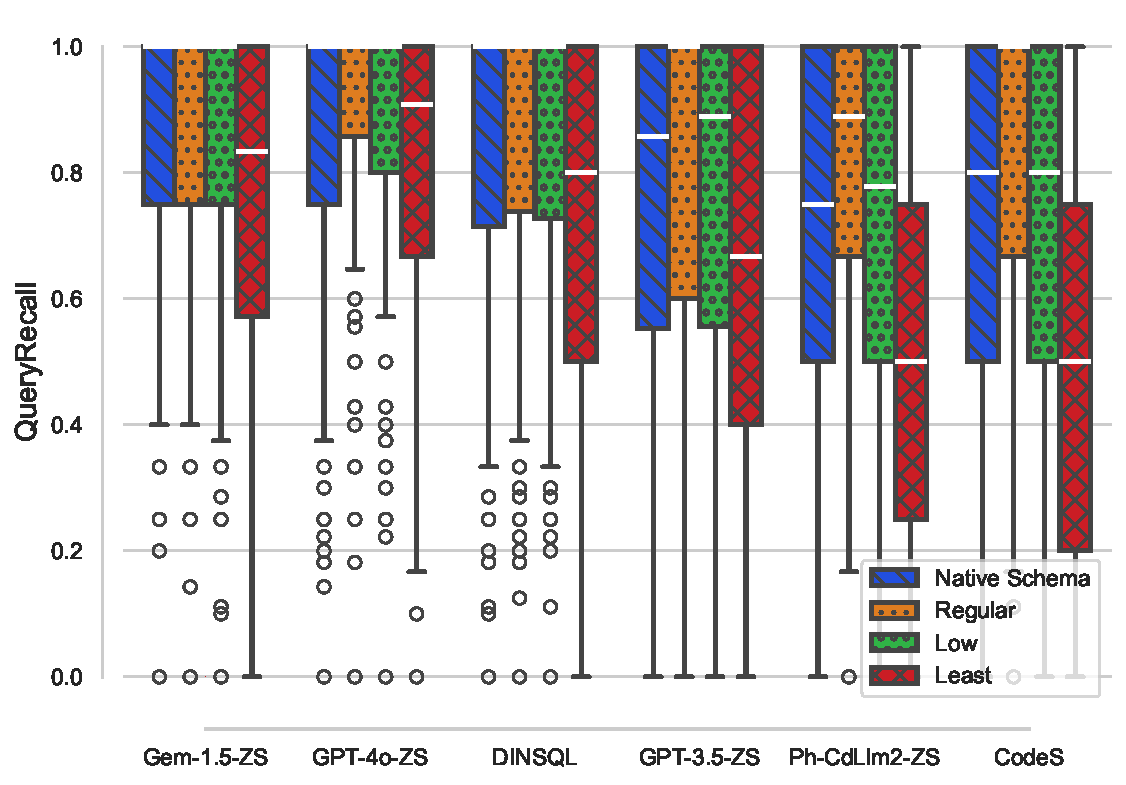
\includegraphics[width=\figwidthmod\linewidth]{figures/recall-boxplot-db-combined.pdf}
  \caption{Schema linking performance across database schema naturalness levels generally yields equal or better performance for higher levels of naturalness, with open source models Phind-CodeLlama2 (Ph-CdLlm2-ZS) and CodeS as well as OpenAI's GPT-3.5 (GPT-3.5-ZS) exhibiting higher sensitivity to changes in naturalness. Zero-shot prompting NL-to-SQL methods are denoted as (ZS).}
  \label{fig:modelrecallnaturalnesslevels}
\end{figure}


Overall, we find that schema naturalness has a model-dependent and significant effect on schema linking performance with the highest correlations between \emph{QueryRecall} and query naturalness occurring with the open-source CodeLlama and CodeS models, and the lowest (though still significant) correlations occurring with Google's SoTA Gemini 1.5 Pro and OpenAI's GPT-4o models.
The more complex DIN SQL and CodeS workflow \emph{QueryRecall} results are also significantly affected by naturalness level differences.

Both DIN SQL and the CodeS complex NL-to-SQL workflows are sensitive to changes in naturalness, suggesting that these more complex workflows by themselves do not overcome schema naturalness effects.  
We also see that execution accuracy differences between the GPT-4o zero-shot prompting method and the DINSQL prompt chaining method suggest that applying more complex workflows to high-performing LLMs may be counterproductive for more recent SoTA LLMs.

Figure \ref{fig:modelrecallnaturalnesslevels} illustrates \emph{QueryRecall} across schema naturalness levels, and for each LLM.
For GPT 3.5, Phind-CodeLlama2, and CodeS, we observe an improvement to \emph{QueryRecall} when converting identifiers in a Native schema to Regular naturalness.
This improvement did not manifest for Gemini and GPT-4o when observing the data in aggregate (i.e., between databases) due to their overall high performance relative to the other models, but improvements within databases of lower naturalness are still present (see Figure \ref{fig:recall-boxplot-dbs}).
The recall drop (approximately 20 percent decrease) associated with a modification from both Regular and Low to Least naturalness remains consistent across all LLMs.

\begin{figure}
  \centering
  \begin{subfigure}{\figwidthmod\linewidth}
    \centering
    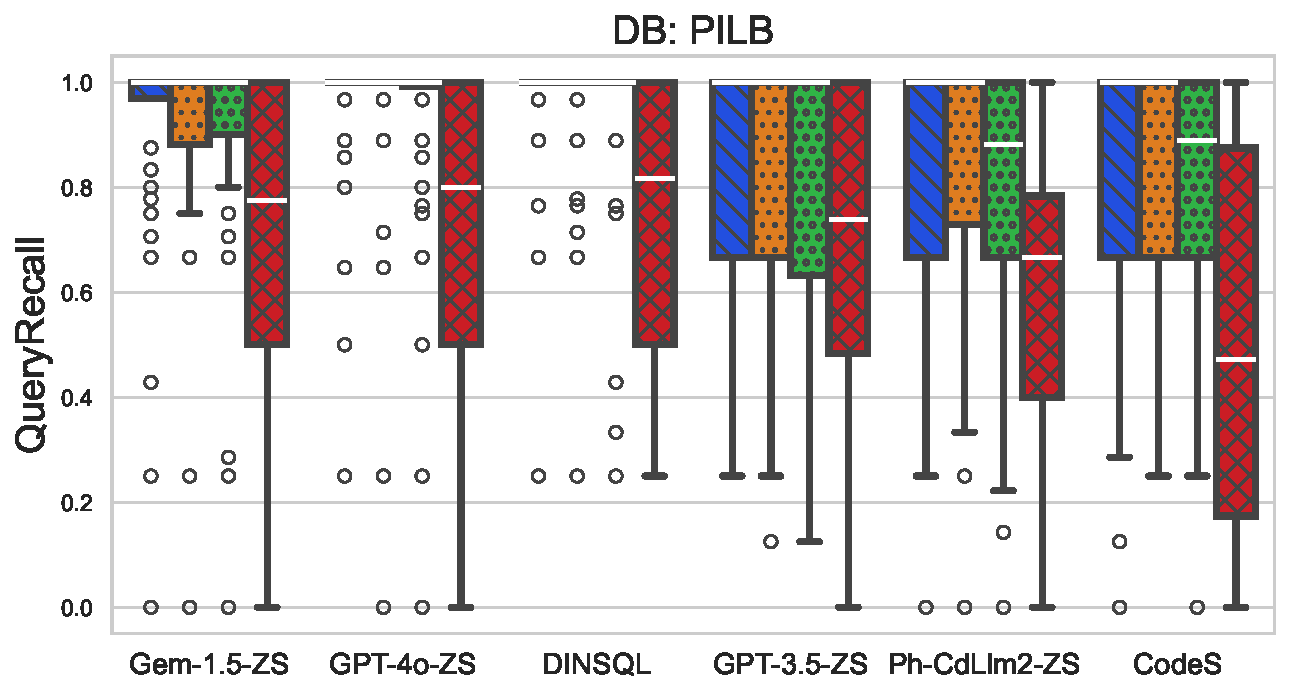
\includegraphics[width=\linewidth]{figures/natlevel-model-recall-boxplot-db-subset-PILB.pdf}
  \end{subfigure}
  \begin{subfigure}{\figwidthmod\linewidth}
    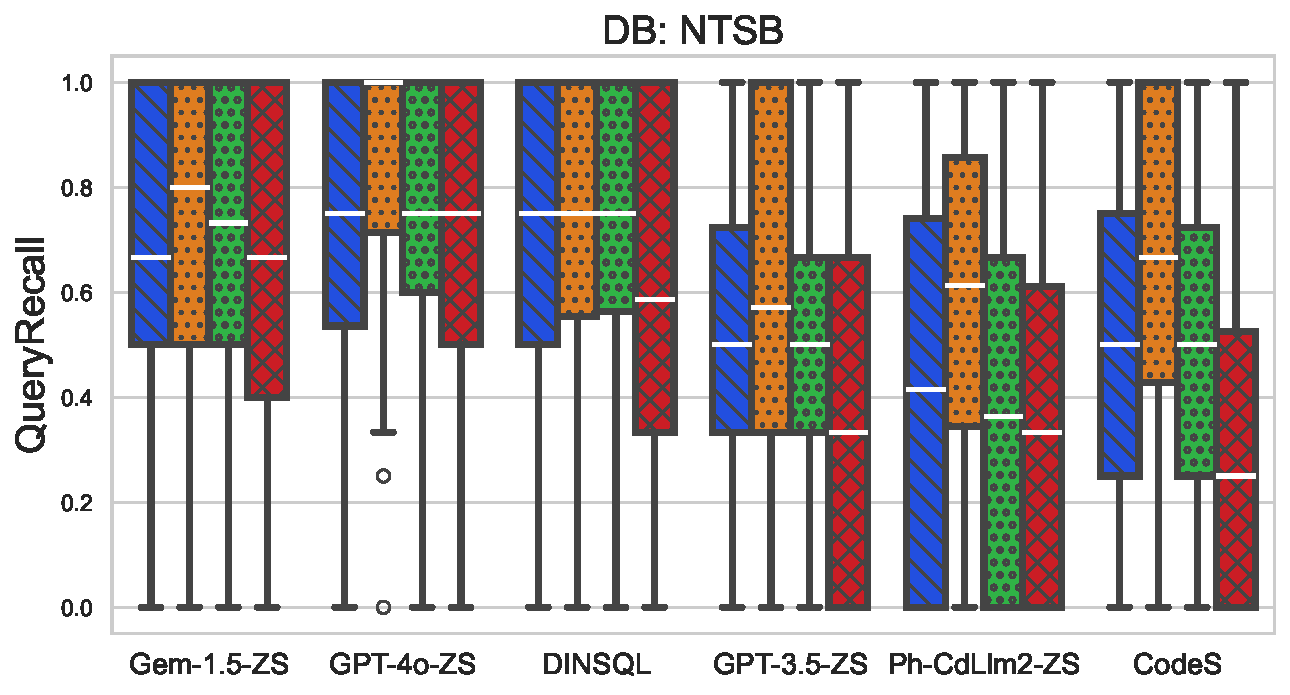
\includegraphics[width=\linewidth]{figures/natlevel-model-recall-boxplot-db-subset-NTSB.pdf}
  \end{subfigure}
  \begin{subfigure}{\figwidthmod\linewidth}
    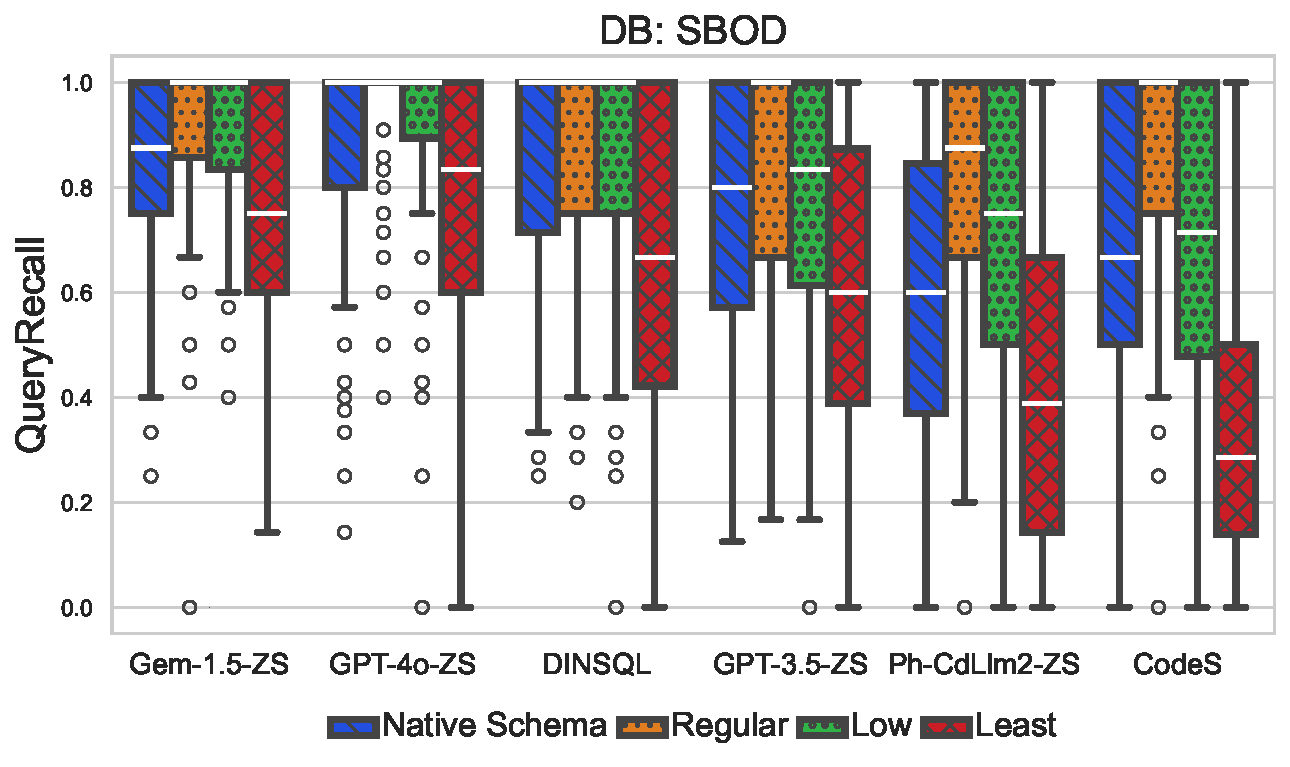
\includegraphics[width=\linewidth]{figures/natlevel-model-recall-boxplot-db-subset-SBOD.pdf}
  \end{subfigure}
  \caption{Schema linking performance (QueryRecall score) changes across 3 example databases' native and virtual schemas. We selected these 3 examples to showcase the diversity of the databases in our collection. PILB Native is a more natural schema with 65 percent Regular, 22 percent Low, and 13 percent Least; NTSB Native contains 42 percent Regular, 34 percent Low, and 24 percent Least; and SBOD Native is the lowest naturalness schema with 24 percent Regular, 49 percent Low, and 27 percent Least.}
  \label{fig:recall-boxplot-dbs}
\end{figure}

Naturalness changes within specific SNAILS database schemas paints a clearer picture of the impact of naturalness.
Figure \ref{fig:recall-boxplot-dbs} provides a drill-down view of the effect of schema modification on the PILB, SBOD, and NTSB schemas in terms of \emph{QueryRecall}, and for each LLM and schema naturalness level.
The center example (PILB) is a highly natural Native schema where schema naturalness modification would not be required. The leftmost example (NTSB) indicates linking performance improvement across all models for a native schema of lower naturalness converted to a higher naturalness schema, and presents a case where naturalness modification will improve NLI performance. The rightmost database (SBOD) represents a Least naturalness schema, and transformation from Native to Regular yields significant improvements for all models. In all cases, we see that reducing naturalness to the Least level consistently degrades \emph{QueryRecall}. 

\paragraph{\textbf{Statistical Significance}}
Kendall-Tau correlations between the proportion of Least identifiers and \emph{QueryRecall} range from $\tau=-0.16$ (Gemini) to $\tau=-0.28$ (Phind-CodeLlama2), with $P < 0.001$ for all models.
Both Regular and Low identifier proportions are significantly correlated with improved outcomes in terms of \emph{QueryRecall}.
Identifiers with Regular naturalness show the highest positive Kendall-Tau correlations ranging from $\tau=0.07$ (Gemini) to $\tau=0.20$ (Phind-CodeLlama2).
Low naturalness identifier proportions correlate positively, but to a lesser degree, with Kendall-Tau values ranging from $\tau=0.05$ (Phind-CodeLlama2) to $\tau=0.07$ (Gemini).

\begin{figure}
  \centering
  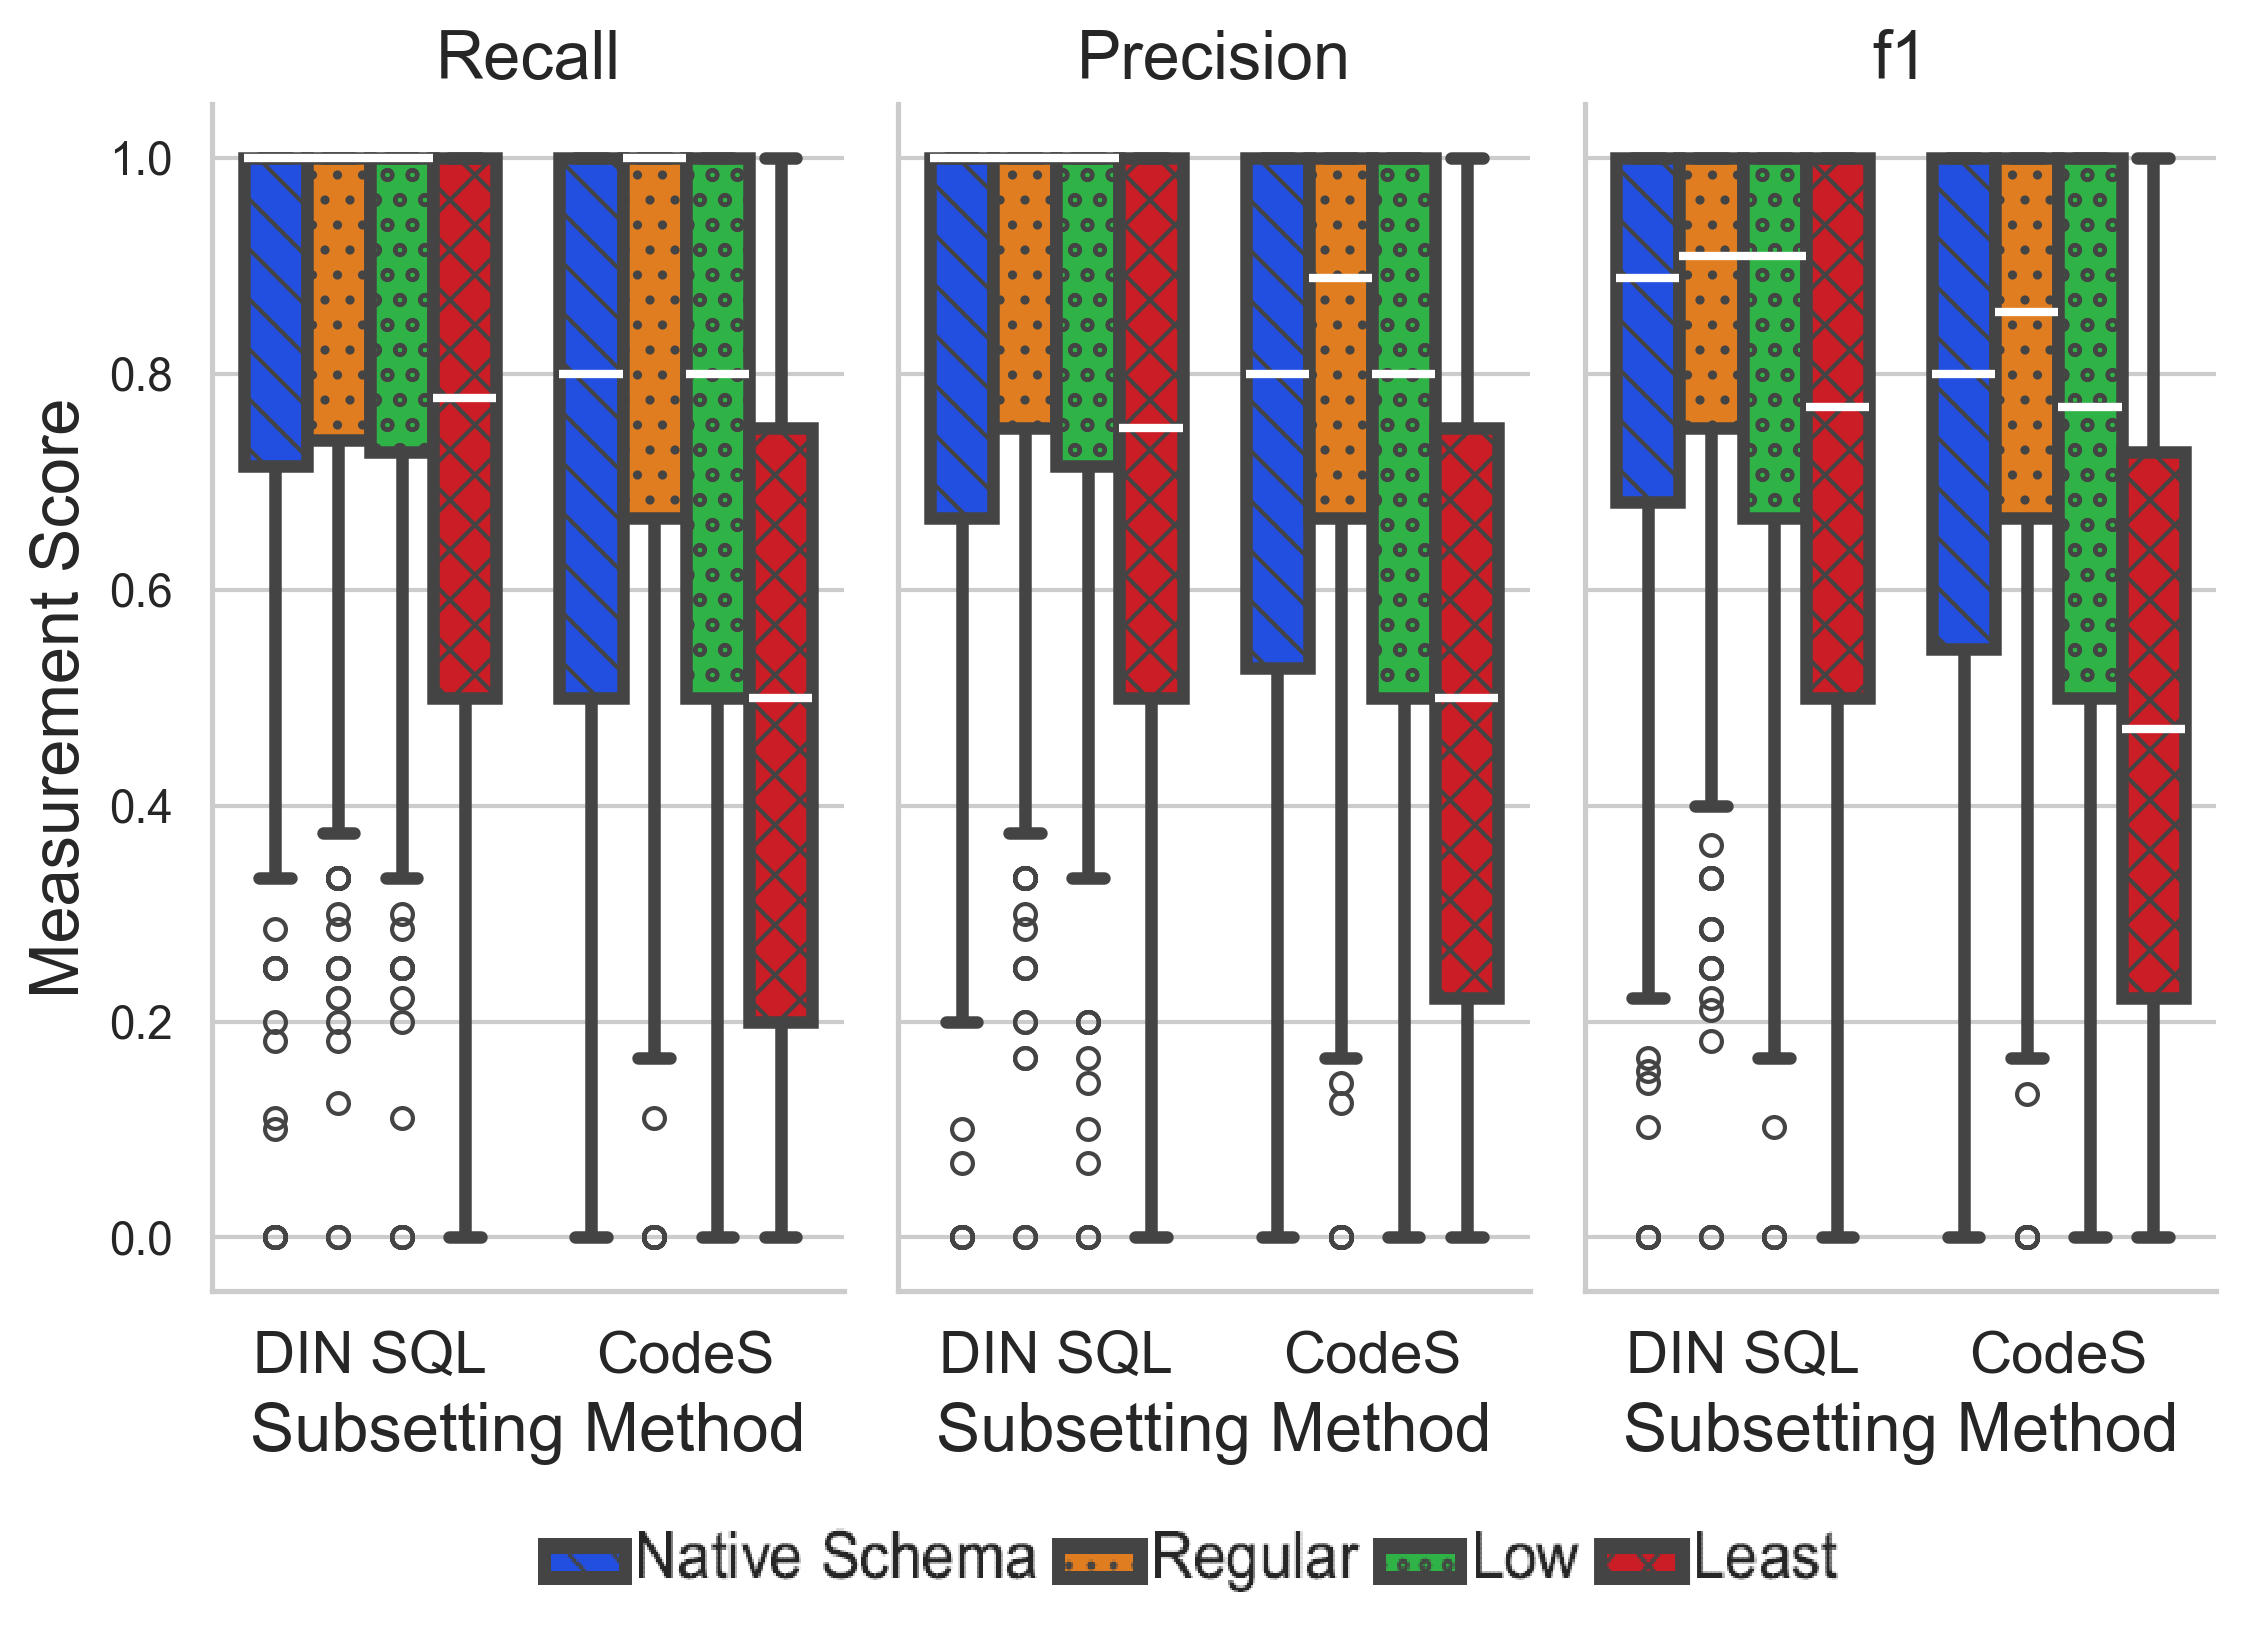
\includegraphics[width=\figwidthmod\linewidth]{figures/dinsql_codes_subsetting_performance.png}
  \caption{Schema subsetting performance, measured with recall, precision, and  f1 score, varies by naturalness levels for both DIN SQL and CodeS. Measurement Score is Recall, Precision, or f1 respectively.}
  \label{fig:subsettingperformance}
\end{figure}

\paragraph{\textbf{Naturalness Effects on Schema Subsetting}}
We measure the schema subsetting (also known as schema filtering, or table retrieval) in terms of recall, precision, and f1 score, and present the results in Figure \ref{fig:subsettingperformance}.
We find that for the CodeS finetuned classifier approach, schema naturalness level differences result in observable differences in f1.
For the DIN SQL LLM-based approach, naturalness effects are less pronounced, though still present, particularly for Least level schemas.

\paragraph{\textbf{Performance Over Modified Spider Schemas}}
Figure \ref{fig:spiderresults} shows that with the SNAILS schema renaming artifacts applied to the Spider NL-to-SQL benchmark dev dataset~\cite{Yu&al.18c}, naturalness effects are the most significant between Low and Least levels of naturalness.
Performance differences across naturalness levels for the highly natural Spider schemas resemble performance over similarly-natural schemas in the SNAILS collection.

\begin{figure}
  \centering
  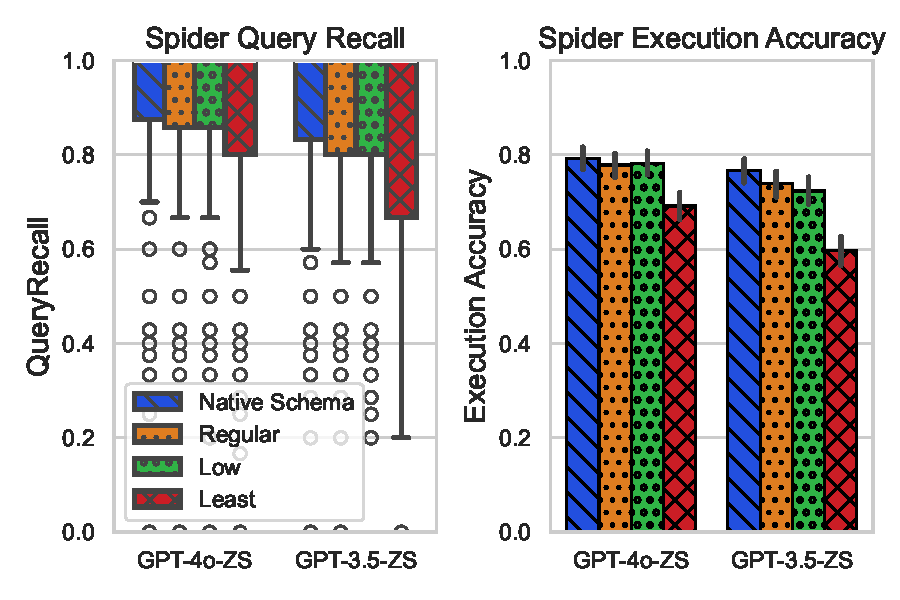
\includegraphics[width=\figwidthmod\linewidth]{figures/spider-combined-results.pdf}
  \caption{QueryRecall and Execution Accuracy differences over the Spider~\cite{Yu&al.18c} dev set modified using SNAILS renaming artifacts.}
  \label{fig:spiderresults}
\end{figure}

\paragraph{\textbf{Additional Charts and Figures}}
The \iftechreport{appendix }\else{technical report~\cite{techreport} }\fi also provides additional fine-grained results: a more detailed tabular breakdown of execution accuracy by schema and LLM; Precision- and F1-based results; token ratio correlations; and more granular \emph{QueryRecall} correlations and box plots.


\section{Discussion and Limitations}


The ability to assess the naturalness of existing schemas can inform the feasibility of ``hooking up'' an NL query interface to an existing database.
We believe that practitioners who are considering the integration of an LLM into their database interaction workflows would benefit from making naturalness-focused schema analysis a key step in their integration process.

\paragraph{\textbf{Other Naming Patterns in Real-World Schemas}}
To examine naming practices in the real-world, we classified the identifiers of SchemaPile dataset~\cite{doehmen2024schemapile} with our CANINE-based classifier, and evaluated the identifiers for other LLM-unfriendly patterns.
We observe that whitespace characters within schema identifiers contributes to identifier mutation during inference.
That is, rather than encasing a whitespace-containing identifier with brackets or quotes, the LLM hallucinates the identifier into snake or camel case format.
We find that in the SchemaPile collection, though whitespace is uncommon (less than 1 percent for both tables and columns), it appears in 808 columns and 63 tables, and is comparable to the proportions in the SNAILS dataset.

Another naming practice that yields disproportionate failures with some LLMs is the presence of the word \emph{table} in the identifier name.
In these instances, we find that the LLM tends to drop the word \emph{table} from the name (e.g., table\_employee becomes employee).
There are over 700 identifiers (less than 1 percent of all identifiers) in the SchemaPile collection that employ this naming pattern.

These observations suggest that although these naming patterns are not necessarily a common occurrence in many real-world schema designs, they do appear in some cases. 
We suggest that practitioners would benefit from assessing the naming patterns of their database schemas.


\paragraph{\textbf{Variations in LLM Sensitivity to Naturalness}}
There are many LLMs to select from for NLIDBs, and we can see even within the select 5 models in our work large variations in NL-to-SQL performance as well as the degree of sensitivity to schema naturalness.
The Google Gemini and GPT-4o models demonstrate the highest overall performance, as well as the lowest sensitivity to naturalness differences between Regular and Low levels.
Without access to the underlying model architectures and weights, it remains as a black box in our research, and we can merely speculate the reasons why it is not as affected by naturalness as the other 3 models in our study.
Generally, we observe that the these models have an overall higher performance, and are less prone to linking errors such as selecting the incorrect identifier from the schema knowledge representation or committing a typo-like hallucination.

Though selecting the most performant model would seem to be an obvious course of action, competing factors such as an organization's policies, budget, or existing vendor contracts, may require the selection of a model that is more sensitive to schema naturalness differences. 
Thus, we believe that naturalness-aware NLI integration will remain important for at least the practitioners who use LLMs other than Gemini in the set that we have studied.


\paragraph{\textbf{Modifying Existing Schemas}}
For already-existing schemas, renaming identifiers is generally a non-trivial effort, particularly for those databases for which documentation has been published and application interfaces have been integrated.
Schema modifications may not be necessary (or helpful), if a schema is already classified as highly natural.
DBAs should assess current naturalness levels prior to committing to naming modifications.
At a minimum, we recommend that any Least identifier be modified to a Regular naturalness level and, if feasible, Low identifiers as well.
If renaming a less natural schema's identifiers is not feasible due to integration constraints, we suggest one of two approaches: 1) adopting a naturalness-as-a-view strategy by mapping Native identifiers to Regular naturalness identifiers using SQL views, or 2) a middleware approach that modifies schema knowledge in LLM prompts and generated SQL queries prior to execution on the database.
We sketch a rough design of both options in the \iftechreport{appendix}\else{technical report~\cite{techreport}}\fi.

We demonstrate a natural schema view proof of concept with our SNAILS database collection and their MS SQL Server instances.
For each table and column in the collection's database schemas, we map the Native table or column to its Regular counterpart in the naturalness modified identifier dataset using SQL view creation DDL and a db\_nl schema.
This enables schema information retrieval for LLM-based NL-to-SQL prompting without prompt or generated query modification while still retaining the underlying Native schema naming patterns required for existing integrations.

In lieu of schema modificaftion, practitioners may elect to employ prompting techniques that augment schema representations with additional metadata or value samples.
While these methods may improve schema linking performance in some contexts~\cite{nan2023enhancingfewshottexttosqlcapabilities}, they greatly increase schema representations on a per-identifier basis.
Thus, the cost to do so is high in terms of token efficiency, latency, and implementation complexity, especially for very large schemas.

\paragraph{\textbf{Designing New Schemas}}
For new schema development, our results show that making schema identifiers more natural from the start can make databases work better with LLMs.
Specifically, database designers should try to avoid Least naturalness identifiers and would likely also benefit from limiting Low naturalness identifiers.
Database practitioners can evaluate the naturalness of identifiers using the identifier naturalness classification techniques and model artifacts described in this paper and released publicly by us as part of the SNAILS collection.

\paragraph{\textbf{Limitations}}
LLM research is advancing rapidly, and the LLMs represented in this paper may get superseded by newer versions or newer models (e.g., DBRX~\cite{dbrx}, Arctic~\cite{snowflakearctic}).
But it does not negate our work's core value--the first in-depth characterization of how schema naturalness affects LLM-based NL-to-SQL--and our new labeled datasets, AI artifacts, and benchmarking framework can be used for future LLMs too.
We leave it to future work to also include such very recent LLMs for further benchmark analyses.

We recognize that the correlation statistics indicate a moderate (in some cases only a weak) correlation between naturalness and \emph{IdentifierRecall}.
This suggests that other undiscovered factors also influence linking performance; and further research may reveal additional schema- and language-related correlations.

Our selection of 9 database schemas is of course not fully representative of \emph{all} types of schemas available in the real-world.
The SNAILS collection will benefit from continued growth in terms of both databases and NL-SQL pairs.
We hope our open source datasets and artifacts can be built upon by the database and NLP communities to keep improving LLM-based NL-to-SQL.

\paragraph{\textbf{Future Work}}
In addition to extending the SNAILS  benchmark artifacts to include additional datasets and artifacts, we identify several NLP+DB directions for future work.
First, we wish to ask why and how exactly do different naturalness levels alter schema linking performance so much?
Is it due to the tokenization and embedding mechanics?
If so, where in the latent space do these altered tokens end up, and how do the encoders make use of them?
Second, why do the different foundational LLMs behave so differently?
Is it related to their architectures, tokenization, (pre)training data, post-training finetuning process, or some other factors?
We believe these open questions have the potential to lead to several interesting new lines of research at the DB and NLP intersection.


\section{Related Work}



\paragraph{\textbf{Ontology Mapping}}
Schema modifications and intermediate representations to enhance performance in a specific context extend beyond NL-to-SQL applications.
Mapping relational database schemas to ontologies is an approach used to improve schema-to-schema integration and web application application-database interfaces~\cite{4061430}.
This improves the semantic description of underlying data, which is often a desirable feature in web applications that interact within the semantic web~\cite{7396620}.
While ontological mapping of a relational database can improve performance in this context; we see less evidence that such an approach is useful or necessary in NL-to-SQL applications, though this may serve as a compelling opportunity for future research.

\paragraph{\textbf{NL-to-SQL Benchmarks}}
\emph{Spider}~\cite{Yu&al.18c}, soon to be superseded by a more challenging benchmark for the LLM era, was a popular NL-to-SQL benchmark that still offers a publically-available dataset consisting of 166 multi-table databases and 1,034 NL questions and gold queries over the databases in a development dataset. 
\emph{Spider-Syn}~\cite{gan-etal-2021-towards} and Spider-Realistic~\cite{gan-etal-2021-towards} are extensions of the Spider benchmark that perform NL question synonym replacement to reduce the occurrences of lexical matching between NL question keywords and schema identifiers.
\emph{BIRD}~\cite{li2023llm} is an emergent benchmark containing 95 large databases over 37 domains that seeks to better replicate real-world databases in order to better challenge highly capable LLM-based NL-to-SQL systems.
While Spider and its variants as well as BIRD intend to better-replicate real-world database designs, our naturalness-focused analysis indicates that their schema identifiers are more natural than those we encountered in our real-world database selection process (see the statistics in Figure \ref{fig:naturalnesscompare}).
Additionally, Spider and BIRD both evaluate performance using either exact set matching or execution result set comparison while we use the more pragmatic set-superset matching as proposed in~\cite{floratou2024nl2sql} and schema linking-specific recall metrics.

\emph{Archerfish}
~\cite{floratou2024nl2sql} is a benchmarking framework that relaxes execution matching and accounts for semantic ambiguity in NL questions by allowing for multiple correct answers derived from candidate key analysis.
This framework relies on the binary ``correct, or not'' evaluation approach common to other benchmarks, whereas in addition to relaxed execution matching, SNAILS evaluates target schema linking performance via query identifier recall.
Overall, we find that our benchmark and findings complement this existing and ongoing research by enhancing our ability to target specific schema-related aspects of NL-to-SQL performance in future NLI development.

\paragraph{\textbf{Impacts of Schema on NL-to-SQL Performance}}
Spider-Syn~\cite{gan-etal-2021-towards} demonstrates degraded NL-to-SQL performance of language models trained for NL-to-SQL tasks when the occurrence of lexical matching between NL questions and schema identifiers is reduced. 
This approach differs from our experiments in that it evaluates a LM specifically trained on NL-to-SQL tasks using the Spider training set as opposed to the more general-purpose foundational LLMs evaluated in this work.
They also make no apparent attempt to reduce the naturalness of  database schema identifiers.

Semantics-preserving schema transformation is a design feature of MT-teql~\cite{10.14778/3494124.3494139}, an NL-to-SQL evaluation framework that modifies natural language utterances and schema properties to stress LM robustness.
MT-teql provides a holistic view of the effect of NL utterance variances and schema design on LM performance. 
However, it does not address the question of schema identifier naturalness, nor does it make modifications to schema elements that are necessary for answer generation. 

Some recent work has examined the effects of schema ambiguity, where semantically different tables or columns have identical or synonymous names.
Schema ambiguity, where a schema contains one or more semantically similar pairs of elements, degrades semantic parsing (i.e., NL-to-SQL) performance by recalling undesired tables or columns in response to a NL question that contains patterns or keywords that align with more than one schema element in the latent space~\cite{10555063}.
Documentation, combined with agent-based column selection, can improve Text-to-SQL performance in the presence of data and schema ambiguity~\cite{huang2023data}.
Though we did not focus on ambiguity in our work, identifier naturalness and ambiguity are complementary efforts that provide a potential future direction for the expansion of the SNAILS benchmark artifacts. 

